%%%%%%%%%%%%%%%%%%%%%%%%%%%%%%%%%%%%%%%%%%%%%%%%%%%%%%%%%%%%%%%%%%%%%%%%%%%%%%%
%
% New interactions of high-energy cosmic neutrinos (working title).
% Skeleton of 2026-11-07: sections, figure placements and the plan's content as
% gray to-do notes; no prose yet (paper/paper_planning.md, Step 6).
%
% Build: pdflatex main && bibtex main && pdflatex main && pdflatex main
%
%%%%%%%%%%%%%%%%%%%%%%%%%%%%%%%%%%%%%%%%%%%%%%%%%%%%%%%%%%%%%%%%%%%%%%%%%%%%%%%

\documentclass[linenumbers, aps, prd, twocolumn, superscriptaddress, floatfix, longbibliography, nofootinbib]{revtex4-2}

\pdfoutput=1
\usepackage{amsmath}
\usepackage{amssymb}
\usepackage{graphicx}
\usepackage{booktabs}
\usepackage{multirow}
\usepackage{placeins}

\usepackage[colorlinks=true,breaklinks=true]{hyperref}
\usepackage[dvipsnames]{xcolor}
\definecolor{darkred}{rgb}{0.5,0,0}
\definecolor{darkblue}{rgb}{0,0,0.5}
\definecolor{firebrick}{rgb}{0.75,0.125,0.125}
\definecolor{darkgreen}{rgb}{0,0.5,0}
\hypersetup{urlcolor=darkblue,
	    citecolor=darkgreen,
	    linkcolor=firebrick}

\usepackage{orcidlink}

\setcounter{topnumber}{3}
\setcounter{dbltopnumber}{2}
\setcounter{bottomnumber}{0}
\renewcommand{\topfraction}{0.95}
\renewcommand{\dbltopfraction}{0.95}
\renewcommand{\textfraction}{0.05}
\renewcommand{\floatpagefraction}{0.8}
\renewcommand{\dblfloatpagefraction}{0.8}

\newcommand{\ie}{{\it i.e.}}
\newcommand{\Ie}{{\it I.e.}}
\newcommand{\eg}{{\it e.g.}}
\newcommand{\Eg}{{\it E.g.}}
\newcommand{\cf}{{\it cf.}}
\newcommand{\etc}{{\it etc.}}
\newcommand{\eq}{Eq.}
\newcommand{\eqs}{Eqs.}
\newcommand{\fig}{Fig.}
\newcommand{\Fig}{Fig.}
\providecommand{\Ref}{}
\AtBeginDocument{\renewcommand{\Ref}{Ref.}}
\newcommand{\Refs}{Refs.}
\newcommand{\Tab}{Table}
\newcommand{\Tabs}{Tabs.}
\newcommand{\equ}[1]{\eq~(\ref{equ:#1})}
\newcommand{\figu}[1]{\fig~\ref{fig:#1}}
\newcommand{\tabl}[1]{\Tab~\ref{tab:#1}}
\newcommand{\MB}[1]{\textcolor{cyan}{[MB: #1]}}
\newcommand{\todo}[1]{\textcolor{gray}{[#1]}}
\newcommand{\placeholder}[1]{\fbox{\parbox{0.9\columnwidth}{\centering\vspace{2.5cm}\todo{#1}\vspace{2.5cm}}}}

\usepackage{array}
\begin{document}

\title{New interactions of high-energy cosmic neutrinos, from the Hubble scale to the Earth}

\author{Mauricio Bustamante\,\orcidlink{0000-0001-6923-0865}}
\email{mbustamante@nbi.ku.dk}
\affiliation{Niels Bohr International Academy, Niels Bohr Institute,\\University of Copenhagen, 2100 Copenhagen, Denmark}

\author{Sudipta Das\,\orcidlink{0000-0002-5508-7751}}
\email{sudipta-das@uiowa.edu}
\affiliation{Department of Physics and Astronomy, University of Iowa, Iowa City, IA 52242, USA}

\author{Sanjib Kumar Agarwalla\,\orcidlink{0000-0002-9714-8866}}
\email{sanjib@iopb.res.in}
\affiliation{Institute of Physics, Sachivalaya Marg, Sainik School Post, Bhubaneswar 751005, India}
\affiliation{Homi Bhabha National Institute, Training School Complex, Anushakti Nagar, Mumbai 400094, India}

\date{\today}

\begin{abstract}
\todo{(1) The question: light mediators of new neutrino interactions act on high-energy astrophysical neutrinos all along their trip.
(2) What we do: follow the flux from the sources through the Universe, the Milky Way, the Sun and the Earth, with the potential and the collisions on the relic neutrinos together, for three families of models.
(3) What we fit: IceCube's flavor composition and spectrum, and its starting and through-going events.
(4) What we find: which stage of the trip matters where, and the resulting limits, with where they compete.
(5) Context: future telescopes.}
\end{abstract}

\maketitle

%%%%%%%%%%%%%%%%%%%%%%%%%%%%%%%%%%%%%%%%%%%%%%%%%%%%%%%%
%%%%%%%%%%%%%%%%%%%%%%%%%%%%%%%%%%%%%%%%%%%%%%%%%%%%%%%%
\section{Introduction}
\label{sec:introduction}

Do neutrinos feel new interactions, carried by light particles that couple to them?
Many extensions of the Standard Model contain such a mediator: a gauge boson of a difference between lepton numbers~\cite{He:1990pn, Foot:1990mn, He:1991qd}, a dark gauge boson that reaches the neutrinos through their mixing with a dark neutrino~\cite{Bertuzzo:2018itn, Jana:2026pwx}, or a scalar or vector through which neutrinos interact among themselves~\cite{Berryman:2022hds}.
Because the mediator is light, its effects reach far.
It can act over long distances, or resonate when neutrinos collide with other neutrinos at specific energies.
Either way, its effects build up over the distance that the neutrinos travel.

Laboratory experiments, neutrino oscillations, and cosmology constrain these mediators strongly over wide ranges of mass and coupling~\cite{Bauer:2018onh, Coloma:2020gfv, Blinov:2019gcj, Escudero:2019gfk, Dror:2020fbh}.
These probes work over terrestrial or solar distances, or in the early Universe, where their reach depends on assumptions about its history.
Effects that accumulate over cosmological distances at high energies lie beyond their reach.
So does a test that is independent of the early Universe.

%%%%%%%%%%%%%%%%%%%%%%%%%%%%%%%%%%%%%%%%%%%%%%%%%%%%%%%%
\begin{figure}[t!]
 \centering
 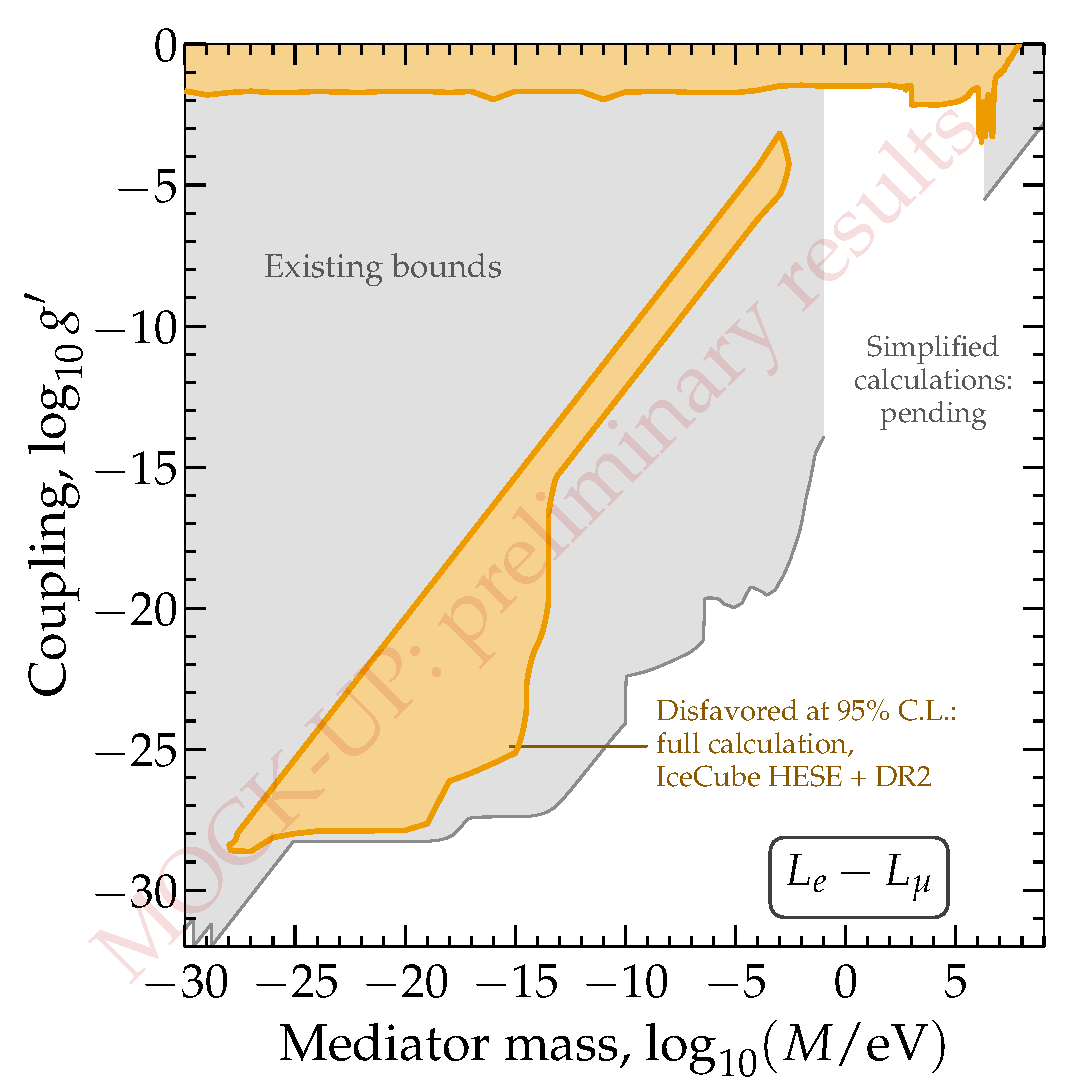
\includegraphics[width=\columnwidth]{figures/mockup_fig1.pdf}
 % mock-up (watermarked, preliminary results; analysis/mockups.py), was: \placeholder{Fig.~1 (money plot): how each stage of the trip moves the limits; $L_e - L_\mu$, IceCube HESE + DR2; full calculation, the potential at the detector only, and one intermediate step; existing bounds in gray.}
 \caption{\textbf{\textit{Limits on $L_e - L_\mu$ from IceCube's starting events and through-going tracks, and how much each stage of the propagation moves them.}} The shaded region is disfavored at 95\%~C.L.\ by the full calculation, which follows the neutrinos from their sources through the Universe, the Milky Way, and the neighborhood of the Sun into the Earth. The curves show the limit when the propagation is simplified: with the potential at the detector only, and \todo{the intermediate step}. Existing bounds are in gray (Table~\ref{tab:bounds}). See Sec.~\ref{sec:results} for details. \todo{Takeaway from the final results: where the full calculation moves the limit, and by how much.}}
 \label{fig:money}
\end{figure}
%%%%%%%%%%%%%%%%%%%%%%%%%%%%%%%%%%%%%%%%%%%%%%%%%%%%%%%%

High-energy astrophysical neutrinos offer such a test~\cite{Ackermann:2022rqc, Arguelles:2022tki}.
Discovered by IceCube~\cite{IceCube:2013low}, they reach the Earth with energies from TeV to PeV, after traveling up to gigaparsecs.
IceCube now measures both their energy spectrum and their flavor composition~\cite{IceCube:2025tgp, IceCube:2025ewu, IceCube:2025ole}.
On their way, a new mediator can act on them through the potential of the matter that they cross, which changes their flavor, and through collisions with the relic neutrinos left over from the early Universe~\cite{Ng:2014pca, Ioka:2014kca}.

Earlier studies treated these effects one at a time and simplified the trip.
Studies of the potential evaluated it only at the detector~\cite{Agarwalla:2023sng}.
Studies of the collisions took the relic neutrinos at rest~\cite{Bustamante:2020mep, Esteban:2021tub}, until a recent one let the lightest of them move~\cite{Wang:2025qap}.

In this work, we follow high-energy neutrinos along their whole trip, through the Universe, the Milky Way, the Sun, and the Earth, computing the potential and the collisions together.
We apply this calculation to the three families of mediators above and fit it to several IceCube data sets: the flavor composition and the spectrum, and the starting and through-going events.
\textbf{How a new mediator changes the flux at Earth depends on where along the trip it acts, so reliable limits need the full trip.}
\todo{Figure~\ref{fig:money} shows \ldots: a paragraph that describes it in full, once the money-plot runs are done.}

Figure~\ref{fig:schematic} shows the trip, as an artist's rendition in four panels that zoom in from one to the next.
In the Universe, the neutrinos travel from their sources through the relic neutrinos, with which they can collide, and through the potential of the Universe's electrons.
In the Milky Way, they cross the potential of its stars and gas, joined by the neutrinos that the Galaxy emits.
Near the Sun, the potentials of the Sun, the Moon, and the Earth switch on.
Inside the Earth, the neutrinos cross its layers on their way to IceCube, at the South Pole.
Of the mediators above, only the gauge boson of a difference between lepton numbers couples to ordinary matter, which sources these potentials; every mediator acts through collisions with the relic neutrinos.

Section~\ref{sec:models} introduces the mediators and the processes through which they act.
Section~\ref{sec:trip} describes the trip, Sec.~\ref{sec:data} the data and the statistical method, and Sec.~\ref{sec:results} our results.
Section~\ref{sec:conclusions} summarizes.
The appendices give the vertices of each model, the transport in full, the flux at the stops of the trip, the thermal rates, the decays in a medium, the transport for secret interactions, and our treatment of the Earth.

%%%%%%%%%%%%%%%%%%%%%%%%%%%%%%%%%%%%%%%%%%%%%%%%%%%%%%%%
\begin{figure*}[t!]
 \centering
 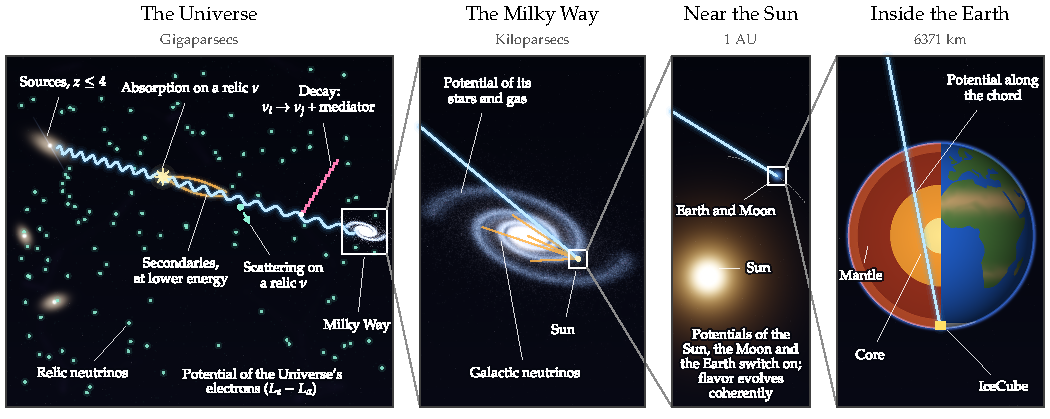
\includegraphics[width=\textwidth]{figures/trip_illustration.pdf}
 \caption{\textbf{\textit{The trip of high-energy astrophysical neutrinos, and what happens along it.}} An artist's rendition, not to scale; each panel zooms in on the next. In the Universe [Eq.~(\ref{equ:transport})], neutrinos from sources out to $z = 4$ can be absorbed on relic neutrinos, which returns secondaries at lower energy, scatter on them, or decay into a lighter neutrino and the mediator, while the potential of the Universe's electrons acts on them for $L_e - L_\alpha$. In the Milky Way [Eq.~(\ref{equ:galactic})], its stars and gas add their potential; the Galaxy also adds its own neutrinos. From the Sun on [Eq.~(\ref{equ:coherent})], the potentials of the Sun, the Moon, and the Earth change the flavor coherently, along each path through the Earth to IceCube. Which of these processes act depends on the model and on the mass of the mediator (Sec.~\ref{sec:models}). See Sec.~\ref{sec:trip} for details.}
 \label{fig:schematic}
\end{figure*}
%%%%%%%%%%%%%%%%%%%%%%%%%%%%%%%%%%%%%%%%%%%%%%%%%%%%%%%%

%%%%%%%%%%%%%%%%%%%%%%%%%%%%%%%%%%%%%%%%%%%%%%%%%%%%%%%%
%%%%%%%%%%%%%%%%%%%%%%%%%%%%%%%%%%%%%%%%%%%%%%%%%%%%%%%%
\section{New light mediators}
\label{sec:models}

In each model that we study, a light particle couples to neutrinos and mediates a new interaction.
We consider three families of such mediators, which act on high-energy neutrinos in different ways.
In the first, a new gauge boson couples to the difference between electron number and muon or tau number~\cite{He:1990pn, Foot:1990mn, He:1991qd}.
This boson couples to electrons as well as to neutrinos, so the electrons in ordinary matter source a potential that changes the flavor of the neutrinos.
In the second, the dark portal, a dark gauge boson reaches the known neutrinos only through their mixing with a new, dark neutrino~\cite{Bertuzzo:2018itn, Jana:2026pwx}.
In the third, secret interactions, a scalar or vector mediator couples to neutrinos alone~\cite{Berryman:2022hds}.
For the latter two, ordinary matter plays no role; only the relic neutrinos act on the high-energy neutrinos, by colliding with them.

Figure~\ref{fig:vertices} shows how the mediator of each model couples to neutrinos: its vertex, with the coupling defined in Eqs.~(\ref{equ:lag_le}), (\ref{equ:lag_dp}), and (\ref{equ:lag_si}).
For Majorana neutrinos, the vertex of a scalar joins two neutrinos.
For Dirac neutrinos, it turns a left-handed neutrino into a right-handed one.

Figure~\ref{fig:processes} shows every process that our calculation includes, built from these vertices, with a vector mediator and, below it, with a scalar one: (a) the potential of ordinary matter; (b) resonant absorption on a relic neutrino; (c, d) scattering on a relic, through the $t$ and $u$ channels; (e) the production of a pair of mediators; (f) the decay of the mediator; (g) the decay of a neutrino into a lighter one and the mediator; and (h) the longitudinal mode of a vector mediator.
Of these, only the potential requires ordinary matter; the rest require only the relic neutrinos.

\subsubsection{\texorpdfstring{$L_e - L_\alpha$}{Le - Lalpha}}
Under the symmetry $L_e - L_\alpha$, with $\alpha = \mu$ or $\tau$, the new boson $Z'$, of mass $M$, couples with strength $g'$ to the electron and its neutrino, and with the opposite sign to the charged lepton $\ell_\alpha$ and its neutrino:
\begin{equation}
 \label{equ:lag_le}
 \begin{split}
 \mathcal{L}_{L_e - L_\alpha} = -g' Z'_\mu \big( & \bar e \gamma^\mu e + \bar\nu_e \gamma^\mu P_L \nu_e \\
  & - \bar\ell_\alpha \gamma^\mu \ell_\alpha - \bar\nu_\alpha \gamma^\mu P_L \nu_\alpha \big) \;,
 \end{split}
\end{equation}
where $P_L$ projects onto left-handed states.
A neutrino at position $\mathbf{r}$ feels the potential of the electrons within a distance of about $1/M$, the range of the interaction [Fig.~\ref{fig:processes}(a)]~\cite{Agarwalla:2023sng}:
\begin{equation}
 \label{equ:potential}
 \begin{split}
 \mathbf{V}(\mathbf{r}) &= g'^2\, \Phi_e(\mathbf{r})\, \mathbf{S}_\alpha \;, \\
 \Phi_e(\mathbf{r}) &= \int d^3 r'\, n_e(\mathbf{r}')\, \frac{e^{-M |\mathbf{r} - \mathbf{r}'|}}{4\pi |\mathbf{r} - \mathbf{r}'|} \;,
 \end{split}
\end{equation}
where $n_e$ is the number density of electrons, $\mathbf{S}_\mu = {\rm diag}(1, -1, 0)$ and $\mathbf{S}_\tau = {\rm diag}(1, 0, -1)$ in the flavor basis.
Antineutrinos feel $-\mathbf{V}$.
The electrons of the Universe, of the Milky Way, of the Sun, of the Moon, and of the Earth all contribute.
Each body contributes once the range reaches it, so the lighter the mediator, the more distant the matter that the neutrinos feel.
Above twice the electron mass, the mediator also decays into charged-lepton pairs [Fig.~\ref{fig:processes}(f)].

\subsubsection{The dark portal}
In the dark portal, no Standard Model particle carries charge under the new gauge symmetry, $U(1)_D$.
A dark neutrino carries it and mixes with the known neutrinos.
The dark gauge boson, $Z_D$, has mass $M$ and coupling $g_D$.
It reaches the known neutrinos through the mixing of the dark neutrino with each flavor $\alpha$, $U_{\alpha 4}$~\cite{Bertuzzo:2018itn, Jana:2026pwx}:
\begin{equation}
 \label{equ:lag_dp}
 \begin{split}
 \mathcal{L}_{\rm DP} &= -Z_{D\mu} \sum_{\alpha\beta} G_{\alpha\beta}\, \bar\nu_\alpha \gamma^\mu P_L \nu_\beta \;, \\
 G_{\alpha\beta} &= g_D\, U_{\alpha 4} U^*_{\beta 4} \;.
 \end{split}
\end{equation}
The coupling matrix $G$ has rank one.
We let the dark neutrino mix with one flavor at a time, so that the interaction has strength $g_D |U_{\alpha 4}|^2$ on $\nu_\alpha$.
In the model of Ref.~\cite{Jana:2026pwx}, $Z_D$ also mixes with the $Z$ boson, which would let matter source a potential, as for $L_e - L_\alpha$.
That mixing is at most $(v_\varphi / v_H)(M / m_Z)$, which follows from Eq.~(6) of Ref.~\cite{Jana:2026pwx} and the structure of its gauge sector.
Here, $v_\varphi$ and $v_H$ are the vacuum values of the Higgs doublets with and without dark charge, and $m_Z$ is the mass of the $Z$ boson.
Their ratio, $v_\varphi / v_H$, is at most a few.
At the light masses where a potential could act, this bound lies 8 to 30 orders of magnitude below the mixing that IceCube data could detect.
We set the mixing to zero, so only the relic neutrinos act on the high-energy neutrinos.

\subsubsection{Secret interactions}
Here a new mediator couples to neutrinos alone, with a flavor structure set by a matrix $G$.
A scalar, $\phi$, and a vector, $V$, couple as
\begin{equation}
 \label{equ:lag_si}
 \begin{split}
 \mathcal{L}_\phi &= -\kappa\, \phi \sum_{\alpha\beta} G_{\alpha\beta}\, \bar\nu_\alpha \nu_\beta \;, \\
 \mathcal{L}_V &= -V_\mu \sum_{\alpha\beta} G_{\alpha\beta}\, \bar\nu_\alpha \gamma^\mu P_L \nu_\beta \;,
 \end{split}
\end{equation}
with $\kappa = 1/2$ for Majorana neutrinos and $\kappa = 1$ for Dirac neutrinos.
We take $G$ equal to $g$ times ${\rm diag}(1, 0, 0)$, ${\rm diag}(0, 1, 0)$, ${\rm diag}(0, 0, 1)$, or the identity, so that the mediator couples with strength $g$ to one flavor or to all of them equally.
With two mediators and two kinds of neutrino, these choices give 16 models.
For Dirac neutrinos, the scalar flips chirality: each vertex joins a left-handed neutrino, which interacts weakly, to a right-handed one, which does not.
Collisions then turn part of the high-energy flux into right-handed neutrinos, which IceCube cannot detect.
Dirac relic neutrinos also keep the helicity they had when they decoupled, so moving relics present the two helicities in unequal proportions (Appendix~\ref{app:thermal}).

\subsubsection{Mass regimes}
The mass of the mediator decides which of the processes in Fig.~\ref{fig:processes} matter.
A high-energy neutrino of energy $E$ meets a relic neutrino of mass $m_r$ at resonance when $E = M^2/(2 m_r)$.
For mediator masses of roughly a keV to tens of MeV, this resonance falls inside IceCube's energy range for at least one relic mass state, depending on the neutrino masses.
For instance, for $M = 10$~MeV, the resonances on the two heavier relics fall at 1.0 and 5.8~PeV.
There, absorption carves dips in the spectrum [Fig.~\ref{fig:processes}(b)], while the decays of the mediator return neutrinos of lower energy [Fig.~\ref{fig:processes}(f)].
For lighter mediators, the high-energy neutrinos also scatter on the relics with small momentum transfer, which moves them between states [Fig.~\ref{fig:processes}(c, d)].
If the mediator is lighter than the difference between two neutrino masses, the heavier neutrino can decay into the lighter one and the mediator [Fig.~\ref{fig:processes}(g)].
For vector mediators, these rates grow as the mediator becomes lighter, through its longitudinal mode.

\subsubsection{Perturbative unitarity}
When the neutrino masses break the symmetry behind the current to which a vector couples, the longitudinal mode of the vector couples to neutrinos like a scalar at energies far above $M$~\cite{Dror:2020fbh}.
For the vectors of Eqs.~(\ref{equ:lag_le}), (\ref{equ:lag_dp}), and (\ref{equ:lag_si}), its couplings to the neutrino mass states $\nu_i$ and $\nu_j$ are~\cite{Allwicher:2021rtd}
\begin{equation}
 \label{equ:goldstone}
 Y_{ij} = \frac{i}{M} \left( G'_{ij}\, m_i + G'_{ji}\, m_j \right) \;,
\end{equation}
where $m_i$ is the mass of $\nu_i$ and $G'$ is the coupling matrix in the basis of mass states [Fig.~\ref{fig:processes}(h)].
These couplings grow as $1/M$.
Tree-level perturbative unitarity requires the largest partial-wave amplitude that they produce to stay below $1/2$ in magnitude~\cite{Allwicher:2021rtd}.
For $L_e - L_\mu$, this excludes $g' > 10^{1.76}\, M/{\rm eV}$ when the lightest neutrino is nearly massless; heavier neutrinos lower this line.
We mark the excluded region in our figures and draw no conclusions from it.
The scalar has no longitudinal mode, so it has no such region.

%%%%%%%%%%%%%%%%%%%%%%%%%%%%%%%%%%%%%%%%%%%%%%%%%%%%%%%%
\begin{figure*}[t!]
 \centering
 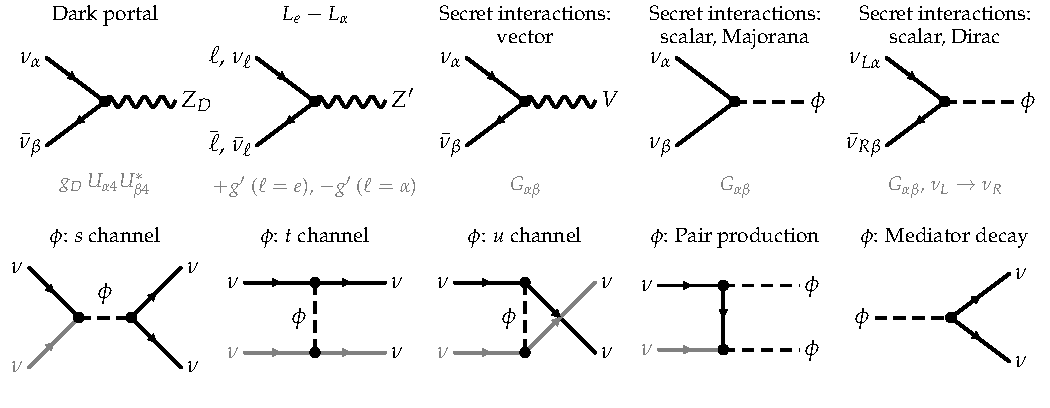
\includegraphics[width=\textwidth]{figures/feynman_vertices.pdf}
 \caption{\textbf{\textit{How the mediator of each model couples to neutrinos.}} Each vertex carries the coupling of Eqs.~(\ref{equ:lag_le}), (\ref{equ:lag_dp}), and (\ref{equ:lag_si}), written under it. Unlike in Fig.~\ref{fig:processes}, the lines carry no arrows of fermion flow. For Majorana neutrinos, a scalar vertex joins two neutrinos; for Dirac neutrinos, it turns a left-handed neutrino into a right-handed one. Because of this, the scalar's absorption in Fig.~\ref{fig:processes}(b) starts from a relic neutrino rather than an antineutrino. See Appendix~\ref{app:vertices} for details.}
 \label{fig:vertices}
 \vspace{0.8em}
 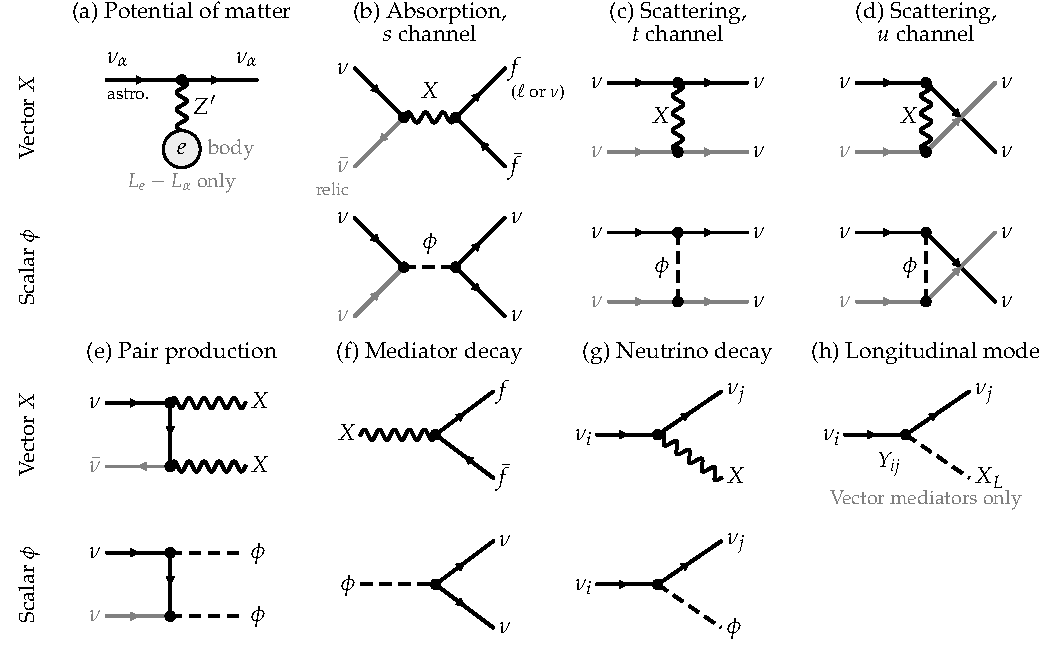
\includegraphics[width=\textwidth]{figures/feynman_processes.pdf}
 \caption{\textbf{\textit{The processes of the trip.}} Every process that our calculation includes, built from the vertices of Fig.~\ref{fig:vertices}. The vector mediator $X$ is $Z'$ for $L_e - L_\alpha$, $Z_D$ for the dark portal, and $V$ for secret interactions; the scalar $\phi$ is that of secret interactions, drawn for Majorana neutrinos. Gray lines are relic neutrinos in every panel. Pair production, (e), proceeds also through the diagram with the two mediators exchanged. Only the potential, (a), needs ordinary matter; every other process needs only the relic neutrinos. See Sec.~\ref{sec:models} for details.}
 \label{fig:processes}
\end{figure*}
%%%%%%%%%%%%%%%%%%%%%%%%%%%%%%%%%%%%%%%%%%%%%%%%%%%%%%%%

%%%%%%%%%%%%%%%%%%%%%%%%%%%%%%%%%%%%%%%%%%%%%%%%%%%%%%%%
%%%%%%%%%%%%%%%%%%%%%%%%%%%%%%%%%%%%%%%%%%%%%%%%%%%%%%%%

\section{Neutrino propagation}
\label{sec:trip}

\subsubsection{Neutrino states}
We follow neutrinos and antineutrinos separately, from their sources to the detector (Fig.~\ref{fig:schematic}).
Over cosmological distances, the phases of their oscillations average out~\cite{Farzan:2008eg}, so the number of neutrinos in each of three states describes the flux fully.
These states are the eigenstates $|a\rangle$, with $a = 1, 2, 3$, of the Hamiltonian
\begin{equation}
 \label{equ:hamiltonian}
 H(E, z) = \frac{U\, {\rm diag}(m_1^2, m_2^2, m_3^2)\, U^\dagger}{2E(1+z)} + \mathbf{V}(z) \;,
\end{equation}
where $U$ is the lepton mixing matrix, $E$ is the energy observed today, $z$ is the redshift, and $\mathbf{V}$ is the potential.
For antineutrinos, $U \to U^*$ and $\mathbf{V} \to -\mathbf{V}^*$.
Without a potential, the eigenstates are the mass states; where the potential dominates, they are nearly pure flavor states.
In normal ordering, $\nu_1$, $\nu_2$, and $\nu_3$ become $\nu_\mu$, $\nu_\tau$, and $\nu_e$ for $L_e - L_\mu$, and $\nu_\tau$, $\nu_\mu$, and $\nu_e$ for $L_e - L_\tau$.
For antineutrinos, the potential has the opposite sign, which exchanges the roles of $\nu_1$ and $\nu_3$.
The cosmological potential varies on the scale of the Hubble time, far more slowly than the neutrinos oscillate, so each neutrino stays in its eigenstate as the potential evolves.
Only collisions and decays move neutrinos between states.
We follow the number of neutrinos in each state until they reach the Sun, where we switch to a coherent description.
We follow three populations: neutrinos, antineutrinos, and, where neutrinos decay, the mediators they emit.

\subsubsection{Sources}
The extragalactic sources lie at redshifts up to $z = 4$, with a comoving number density that tracks the star-formation rate~\cite{Yuksel:2008cu}: it grows as $(1+z)^{3.4}$ up to $z = 1$ and falls as $(1+z)^{-0.3}$ beyond.
We place them in the cosmic mean density of matter, without the matter of their host galaxies, so the potential where they emit is the cosmological one.
Each source emits neutrinos and antineutrinos with the flavor composition of pion decay, $(f_{e,S}, f_{\mu,S}, f_{\tau,S}) = (1/3, 2/3, 0)$, at every energy (Sec.~\ref{sec:data} also fits it).
The ratio of antineutrinos to neutrinos at the sources, $\xi$, is 1, as for proton-proton collisions.
In the fits to event samples and in the forecasts, it is free between 1/2, as for proton-photon collisions, and 1.
There, neutrinos and antineutrinos keep the same flavor composition.
At the source, this mixture of flavors splits incoherently over the eigenstates of Eq.~(\ref{equ:hamiltonian}) at the redshift of the source, each flavor $\nu_\alpha$ contributing to state $a$ in proportion to $|\langle\nu_\alpha|a\rangle|^2$.

IceCube's measured spectrum is softer above a break at 24.5~TeV than below it~\cite{IceCube:2025ewu}.
Without a new interaction, the flux per flavor of neutrinos plus antineutrinos at Earth is then
\begin{equation}
 \label{equ:bpl}
 \Phi(E) = \Phi_{\rm astro} \times
 \begin{cases}
 (E/E_0)^{-\gamma} \;, & E \geq E_{\rm b} \;, \\
 (E_{\rm b}/E_0)^{-\gamma}\, (E/E_{\rm b})^{-\gamma_{\rm low}} \;, & E < E_{\rm b} \;,
 \end{cases}
\end{equation}
with $E_0 = 100$~TeV, the break at $E_{\rm b} = 24.5$~TeV, the normalization $\Phi_{\rm astro}$, and the spectral indices $\gamma$ above the break and $\gamma_{\rm low}$ below it.
We reproduce it with two populations of sources, $j = {\rm up}$ and ${\rm low}$, each emitting a power law in energy with its own index, $\gamma_{\rm up} = \gamma$ and $\gamma_{\rm low}$.
They are separated at the break energy observed today: one supplies only the neutrinos that arrive above $E_{\rm b}$, the other only those that arrive below it.
Split over the eigenstates at the sources, they inject into state $a$, per unit energy observed today, at the rate
\begin{equation}
 \label{equ:source}
 \begin{split}
 \mathcal{S}_a(E, z) = \; & w_\nu\, R(z)\, (1+z) \sum_j K_j\, [E(1+z)]^{-\gamma_j}\, \Theta_j(E) \\
 & \times \sum_\alpha f_{\alpha,S}\, |\langle\nu_\alpha|a\rangle|^2 \;,
 \end{split}
\end{equation}
where $R(z)$ is the comoving density of sources, $w_\nu = 1/(1+\xi)$ and $w_{\bar\nu} = \xi/(1+\xi)$ weigh the two kinds, $(1+z)$ converts the energy at the source into that observed today, and $\Theta_{\rm up}(E) = \Theta(E - E_{\rm b})$ and $\Theta_{\rm low}(E) = \Theta(E_{\rm b} - E)$ select the energies of each population.
The constants $K_j$ are set so that, without a new interaction, the two populations add up at Earth to Eq.~(\ref{equ:bpl}), continuous at the break.
Since the transport is linear in its sources, we solve it for each population separately and add the two solutions.
Likewise, a free $\xi$ needs one more solution, with neutrinos alone.
Every other value of $\xi$ is a combination of the two solutions.
New physics can move neutrinos across the break: absorption above it, for instance, produces secondaries below it, which stay in the solution of the population that emitted their parents.
The normalization and both spectral indices are free in the fits (Sec.~\ref{sec:data}); we interpolate between solutions computed at a few fixed values of each index.
The neutrinos that the Milky Way itself emits are described with the Milky Way, below.

\subsubsection{The transport equation}
From the sources to today, the number $F_a(E, z)$ of neutrinos per unit energy in state $a$ evolves as
\begin{equation}
 \label{equ:transport}
 \begin{split}
 \frac{\partial F_a}{\partial t} = \; & \mathcal{S}_a - \Gamma^{\rm abs}_a F_a + \mathcal{R}_a + \sum_{b \neq a} \left( R_{ab} F_b - R_{ba} F_a \right) \\
 & + \frac{\partial}{\partial E} \left( b_a F_a \right) - \Gamma^{\rm dec}_a F_a + \mathcal{D}_a + \mathcal{M}_a \;,
 \end{split}
\end{equation}
with $dt = -dz / [(1+z) H(z)]$ and $H(z)$ the Hubble rate, for the cosmological parameters of Planck 2018~\cite{Planck:2018vyg}.
The number $\bar F_a$ of antineutrinos obeys the same equation, with each quantity replaced by its counterpart for antineutrinos.
The terms are, in order:
the sources, Eq.~(\ref{equ:source});
absorption on the relics [Fig.~\ref{fig:processes}(b)];
the neutrinos that absorption returns when the mediator decays, $\mathcal{R}_a$ [Fig.~\ref{fig:processes}(f)];
scatterings on the relics with small momentum transfer, which move neutrinos between states without changing their number [Fig.~\ref{fig:processes}(c, d)];
the energy that neutrinos lose in those scatterings when the relic changes its mass state;
the decay of state $a$ into lighter ones by emitting the mediator, and the daughters $\mathcal{D}_a$ that decays feed into it [Fig.~\ref{fig:processes}(g)];
and the neutrinos $\mathcal{M}_a$ that the emitted mediators return when they decay in turn [Fig.~\ref{fig:processes}(f)].

These mediators form the third population.
Their number $N_h(E, z)$ per unit energy, in helicity $h$, evolves as
\begin{equation}
 \label{equ:mediators}
 \frac{\partial N_h}{\partial t} = \mathcal{P}_h - \frac{\Gamma_{\rm med}\, M}{E(1+z)}\, N_h \;,
\end{equation}
where $\mathcal{P}_h$ is the rate at which the decays emit them and $\Gamma_{\rm med}$ is their width at rest into neutrino pairs.
A vector has three helicities and a scalar one.
Three terms couple the neutrinos and the antineutrinos: absorption returns both kinds, a Majorana neutrino that flips its helicity in a decay emerges as an antineutrino, and the mediators decay into pairs of both kinds.
Because $E$ is the energy observed today, the redshift enters through it, with no separate term.
Which terms act depends on the model and on the mass of the mediator.
Table~\ref{tab:terms} shows, for each model, the terms of Eqs.~(\ref{equ:transport}) and (\ref{equ:mediators}) that we include and the masses at which they act.
Only $L_e - L_\alpha$ adds a potential, since only its mediator couples to ordinary matter.
The resonant absorption acts where its energy, $E = M^2/(2 m_r)$, falls among the measured energies, and the decays where the mediator is lighter than the difference between two neutrino masses.
Below 1~keV, the scatterings with small momentum transfer move neutrinos between states, and, for the vectors, cost them energy when the relic changes mass.
At MeV masses, where the potential is negligible, the eigenstates are the mass states.
There we solve it with every channel of Fig.~\ref{fig:processes}(b)--(e), pair production included (Appendix~\ref{app:si}).
Appendix~\ref{app:transport} gives every term in full.

%%%%%%%%%%%%%%%%%%%%%%%%%%%%%%%%%%%%%%%%%%%%%%%%%%%%%%%%
\begin{table*}[t!]
 \caption{\label{tab:terms}\textbf{\textit{The terms of the transport that each model includes, and where they act.}} The terms are those of Eqs.~(\ref{equ:hamiltonian}), (\ref{equ:transport}), and (\ref{equ:mediators}); $m_r$ is the mass of the relic, $m_i - m_j$ the difference between two neutrino masses, and $m_k + m_l$ the sum of two. See Sec.~\ref{sec:trip} and Appendix~\ref{app:transport} for details.}
 \begin{ruledtabular}
 \begin{tabular}{>{\raggedright\arraybackslash}p{0.25\textwidth}>{\raggedright\arraybackslash}p{0.17\textwidth}>{\raggedright\arraybackslash}p{0.17\textwidth}>{\raggedright\arraybackslash}p{0.17\textwidth}>{\raggedright\arraybackslash}p{0.17\textwidth}}
 Term & $L_e - L_\alpha$ ($Z'$) & Dark portal ($Z_D$) & Secret, vector ($V$) & Secret, scalar ($\phi$) \\
 \hline
 Potential, $\mathbf{V}$ & Below 1~keV; electrons of the Universe, the Milky Way, the Sun, the Moon, and the Earth & None & None (it vanishes without a relic lepton asymmetry) & Not modeled; the region where it matters is not used \\
 Absorption, $\Gamma^{\rm abs}_a$, and its secondaries, $\mathcal{R}_a$ & Where $M^2/(2 m_r)$ falls among the measured energies ($M \approx 1$~keV--50~MeV) & Same & Same & Same, on relic neutrinos \\
 Scatterings with small momentum transfer, $R_{ab}$ & Below 1~keV & Below 1~keV & Below 1~keV & Below 1~keV \\
 Scatterings with large momentum transfer and pair production & Above 1~keV; below it, for couplings above $10^{-4}$ & Same & All masses & All masses \\
 Energy loss, $b_a$ & Below 1~keV & Below 1~keV & Below 1~keV & None \\
 Decays, $\Gamma^{\rm dec}_a$ and $\mathcal{D}_a$ & $M < m_i - m_j$ & Same & Same & Same \\
 Decays of the emitted mediators, $\mathcal{M}_a$ and $N_h$ & $m_k + m_l < M < m_i - m_j$ & Same & Same & Same \\
 Longitudinal mode & In the decays; its scatterings below 1~keV & In the decays; its scatterings left out & Same as the dark portal & None \\
 \end{tabular}
 \end{ruledtabular}
\end{table*}
%%%%%%%%%%%%%%%%%%%%%%%%%%%%%%%%%%%%%%%%%%%%%%%%%%%%%%%%

\subsubsection{Absorption on the relics}
State $a$ is absorbed at the rate
\begin{equation}
 \label{equ:absorption}
 \Gamma^{\rm abs}_a(E, z) = \sum_r \Gamma_r(E, z)\, \frac{1}{2} \left| (U^\dagger G W)_{ra} \right|^2 \;,
\end{equation}
where $r$ runs over the relic mass states, $W$ holds the eigenvectors of Eq.~(\ref{equ:hamiltonian}) in the flavor basis, and $\Gamma_r$ is the rate of resonant absorption on relic $r$ per unit coupling.
Thus, the absorption amplitude combines coherently the flavor content of state $a$ and that of relic $r$.
For instance, in vacuum, a coupling equal for all flavors absorbs mass state $j$ only on relic $j$.
We average $\Gamma_r$ over the thermal momenta of the relics, at temperature $T_{\nu,0}(1+z)$, with $T_{\nu,0} = 1.68 \times 10^{-4}$~eV today.
This average matters most when the lightest relic is relativistic, which broadens its resonance~\cite{Wang:2025qap}.
At MeV masses, the thermal motion of the relics enters every collision term, not only the resonance.
For Dirac relics, we also account for their helicity (Appendix~\ref{app:thermal}).
Each absorption of a neutrino of energy $E'$ returns a neutrino and an antineutrino, with energy spectra $3E^2/E'^3$ and $3(E' - E)^2/E'^3$.

\subsubsection{Decays and scatterings}
For light mediators, two more processes move neutrinos between states.
A state can decay into a lighter one by emitting the mediator [Fig.~\ref{fig:processes}(g)]; for Majorana neutrinos, the daughter can also be an antineutrino.
A mediator heavier than two neutrinos decays in turn into a neutrino pair, returning its energy to the flux [Eq.~(\ref{equ:mediators}) and Appendix~\ref{app:decay}].
Scatterings on the relics that transfer little momentum move neutrinos between states without changing their number [Fig.~\ref{fig:processes}(c, d)].
When the relic changes its mass state in such a scattering, the neutrino also loses energy.
In a potential, the states that decay are the eigenstates of Eq.~(\ref{equ:hamiltonian}), not the mass states (Appendix~\ref{app:decay}).
The two processes compound: scatterings refill the states that decay, so together they drain the flux at a given energy more than either does alone.

Figure~\ref{fig:collisions} shows what each term of Eq.~(\ref{equ:transport}) does to the flux at the detector, versus energy, switching the terms on one at a time.
Its top row shows the flux of all flavors over the flux with no new interaction; the rows below show the share of each flavor.
For a 10~MeV scalar coupled to $\nu_\tau$, with $g = 10^{-3}$, the lines add in turn resonant absorption, the other collisions with the relics, and the thermal motion of the relics.
For $L_e - L_\mu$ at $10^{-2}$~eV, with $g' = 10^{-6}$, they add the potential, the decays, and the scatterings on the relics.
On the left, absorption opens a dip at each resonance with a $\nu_2$ or $\nu_3$ relic; the neutrinos that it gives back lift the flux just below.
Adding the scatterings deepens the loss that the decays cause.

\subsubsection{The Milky Way}
Today, the extragalactic flux enters the Milky Way, whose stars and gas~\cite{McMillan:2016jtx} add their own potential to the cosmological one.
This potential also changes slowly along the way, so each state passes smoothly into the matching eigenstate of the potential near the Sun.
Where the potential of the Milky Way opens decays that the cosmological one does not, we instead follow the flux across the Galaxy direction by direction, with the rates of Eq.~(\ref{equ:transport}), along each line of sight [Eq.~(\ref{equ:galactic}) in Appendix~\ref{app:transport}].
The Milky Way also emits neutrinos of its own, made by cosmic rays that collide with its gas and by unresolved sources~\cite{Schwefer:2022zly, IceCube:2023ame}.
We follow them from where they are emitted, along each line of sight, through the same processes.
In the Milky Way, absorption on the relics is negligible: their column is about $10^{-5}$ of the cosmic one.

\subsubsection{The Sun, the Moon, and the Earth}
From the Sun on, we follow the flux coherently: the potentials of the Sun, the Moon, and the Earth switch on over distances comparable to the oscillation lengths, so the phases between states matter.
The density matrix of the flux starts as $\rho = \sum_a N_a |a\rangle\langle a|$, with $N_a$ the number of neutrinos, extragalactic and Galactic, in state $a$, and evolves as
\begin{equation}
 \label{equ:coherent}
 \frac{d\rho}{dx} = -i \left[ H(x), \rho \right] \;,
\end{equation}
where $x$ is the distance along the path and $H(x)$ is the Hamiltonian of Eq.~(\ref{equ:hamiltonian}) today, with the potential of the new interaction at $x$.
At the detector, the flux of flavor $\alpha$ is $\langle\nu_\alpha|\rho|\nu_\alpha\rangle$, averaged over the paths through the Earth from each direction.
Along the way, the potentials of the Sun, of the Moon, and of the Earth itself switch on, each within its range.
Where a potential switches on slowly compared to the oscillations, it turns each state into its own eigenstate.
For instance, for $L_e - L_\mu$ at $10^{-20}$~eV, the potential of the Sun turns the mass state $\nu_2$ into $\nu_\tau$.

Inside the Earth, we compute the potential of $L_e - L_\alpha$ from Eq.~(\ref{equ:potential}), with the electron density of the Preliminary Reference Earth Model~\cite{Dziewonski:1981xy} (Appendix~\ref{app:earth}).
To it we add the charged-current potential of the Standard Model, $\sqrt{2}\, G_F\, n_e$ for $\nu_e$, from the same electron density $n_e$, step by step along each path.
Where the flux arrives as a mixture of mass states, as it does for the dark portal, for secret interactions, and for mediators above 1~keV, we neglect the potential of the Standard Model: it changes the flavor share of a mass state by at most $3.3 \times 10^{-3}$ at 1~TeV, the lowest energy of the present data.
The change falls as $1/E$ above that.
Our transport changes the flavor inside the Earth without removing neutrinos.
The standard absorption in the Earth comes instead from the detector responses (Sec.~\ref{sec:data}), applied to the flavors that arrive.
This is exact where absorption is the same for every flavor, as in the models of the future telescopes.
It is approximate only where flavor changes inside the Earth, under the potential of $L_e - L_\alpha$, and only for the two parts of absorption that depend on flavor: the Glashow resonance of $\bar\nu_e$ at 6.3~PeV and the regeneration of $\nu_\tau$.
In the starting events, these concern at most $3 \times 10^{-4}$ and 10\% of the astrophysical events, respectively (up-going $\bar\nu_e$ between 4 and 10~PeV, and up-going $\nu_\tau$ above 100~TeV).
We neglect collisions and decays from the Sun on; decays would matter there only where the potential already dominates the change of flavor (Appendix~\ref{app:decay}).

Figure~\ref{fig:species} shows the flux of each of the six species, the three flavors of neutrinos and of antineutrinos, position by position along the whole trip, for one benchmark of each family: a 10~MeV scalar coupled to $\nu_\tau$, for secret interactions; a $10^{-2}$~eV mediator mixed with $\nu_\tau$, for the dark portal; and $L_e - L_\mu$ at $10^{-26}$ and $10^{-20}$~eV.
Its four columns match the panels of Fig.~\ref{fig:schematic}: the Universe, versus redshift; a line of sight across the Milky Way; a path past the Sun; and a chord through the Earth.
The sources sit in a shell at $z = 1.8$--$2.2$.
We show one observed energy, 495~TeV, and normalize each flux to the total after the sources stop emitting.
Secret interactions and the dark portal, which have no potential, act only in the Universe.
For $L_e - L_\mu$, the place where the flavor changes depends on the mediator mass: at $10^{-26}$~eV, the Milky Way, whose potential also opens decays between the lightest neutrino and antineutrino states that drain part of the flux; at $10^{-20}$~eV, the neighborhood of the Sun.
Appendix~\ref{app:stops} shows how this depends on energy.

%%%%%%%%%%%%%%%%%%%%%%%%%%%%%%%%%%%%%%%%%%%%%%%%%%%%%%%%
\begin{figure*}[t!]
 \centering
 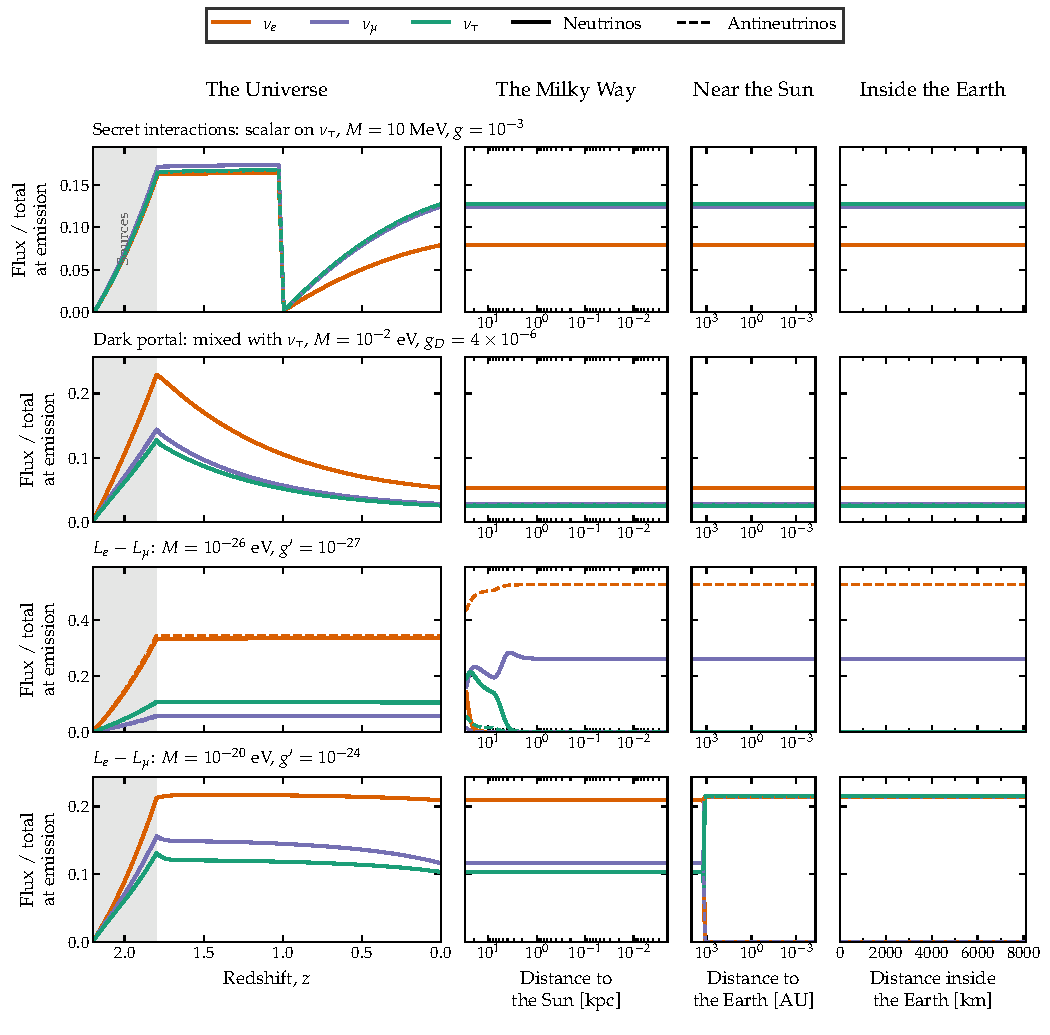
\includegraphics[width=\textwidth]{figures/species_along_trip.pdf}
 \caption{\textbf{\textit{Where along the trip each family of mediators acts.}} The flux of each species, neutrinos and antineutrinos of each flavor, at an observed energy of 495~TeV, from sources in a shell at $z = 1.8$--$2.2$ (gray) to the detector, divided by the total once the sources stop emitting. The columns follow the panels of Fig.~\ref{fig:schematic}: the Universe; one line of sight across the Milky Way; one path past the Sun, perpendicular to the direction to it; and one chord through the Earth, at $\cos\theta_z = -0.64$. Secret interactions absorb the neutrinos resonantly in the Universe, and the secondaries of the absorption partly refill the flux. The dark portal drains it across the Universe through decays and scatterings on the relic neutrinos. For $L_e - L_\mu$, the potential of the Milky Way opens decays that turn neutrinos into antineutrinos at $10^{-26}$~eV; that of the Sun turns the states into flavor states at $10^{-20}$~eV. Inside the Earth, nothing changes at these energies.}
 \label{fig:species}
\end{figure*}
%%%%%%%%%%%%%%%%%%%%%%%%%%%%%%%%%%%%%%%%%%%%%%%%%%%%%%%%
%%%%%%%%%%%%%%%%%%%%%%%%%%%%%%%%%%%%%%%%%%%%%%%%%%%%%%%%

%%%%%%%%%%%%%%%%%%%%%%%%%%%%%%%%%%%%%%%%%%%%%%%%%%%%%%%%
\begin{figure*}[t!]
 \centering
 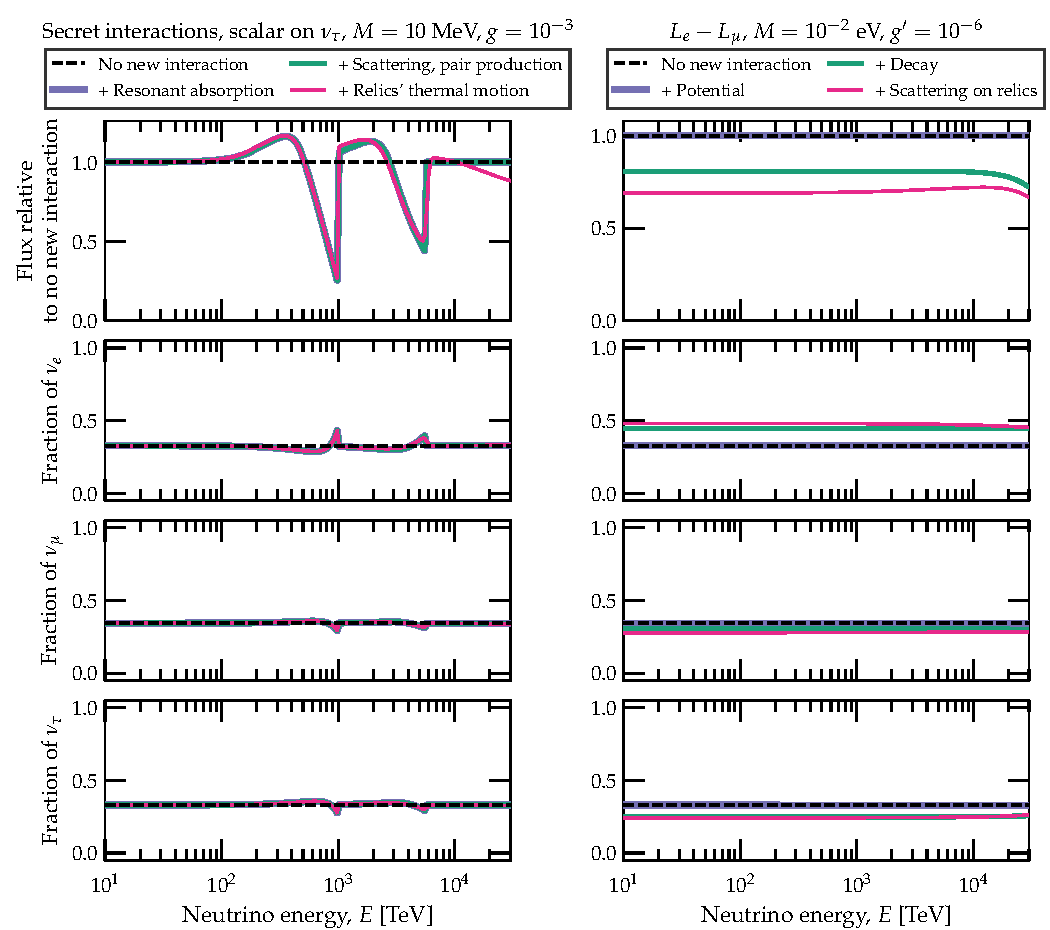
\includegraphics[width=\textwidth]{figures/collision_terms.pdf}
 \caption{\textbf{\textit{What each term of the transport does to the flux and its flavors.}} \textit{Top:} the all-flavor flux, relative to that without a new interaction. \textit{Below:} the share of each flavor. Each line adds one term to those of the line before. We assume pion-decay sources, $\nu_e : \nu_\mu : \nu_\tau = 1 : 2 : 0$, with an $E^{-2.5}$ spectrum, the normal mass ordering, and the lightest neutrino at $10^{-6}$~eV. \textit{Left:} absorption carves dips where the neutrinos resonate with the $\nu_2$ and $\nu_3$ relics, while the neutrinos it returns raise the flux below each dip. \textit{Right:} scatterings on the relics, which alone conserve the number of neutrinos, deepen the loss from decays. See Sec.~\ref{sec:trip} for details.}
 \label{fig:collisions}
\end{figure*}
%%%%%%%%%%%%%%%%%%%%%%%%%%%%%%%%%%%%%%%%%%%%%%%%%%%%%%%%

%%%%%%%%%%%%%%%%%%%%%%%%%%%%%%%%%%%%%%%%%%%%%%%%%%%%%%%%
%%%%%%%%%%%%%%%%%%%%%%%%%%%%%%%%%%%%%%%%%%%%%%%%%%%%%%%%
\section{Data and statistical method}
\label{sec:data}

\subsubsection{Data}
Table~\ref{tab:data} lists the data sets, which we fit each on its own.
The first is IceCube's published measurements of the diffuse flux: its flavor composition and its energy spectrum.
For the flavor composition, IceCube released its likelihood as a function of $(f_e, f_\mu)$, measured with its medium-energy starting events~\cite{IceCube:2025ole}.
IceCube computed it assuming the broken power law of its own spectral fit.
The measured composition is that of the detected neutrinos, so it depends on how often the detector records each flavor.
We therefore compare it with the composition of our flux over the same energies, 5~TeV--10~PeV, with each flavor weighted by the number of starting events it would produce.
We compute these numbers with the effective areas of the release.
For the spectrum, IceCube gives the normalization of an $E^{-2}$ flux in each of ten energy segments~\cite{IceCube:2025ewu}.
In each segment, we compute the normalization of the $E^{-2}$ flux that holds as many neutrinos as our flux.
Our flux here is the extragalactic one plus the Galactic one, averaged over the sky, since IceCube's measured flux includes the Galactic plane.
IceCube's normalizations are instead those that best fit its events.
Computing them in the same way would need IceCube's detector response, which is not public.
To gauge the difference, we fit IceCube's broken power law to the segments with our normalizations.
Its normalization comes out $0.9\sigma$ lower than in IceCube's fit, and its upper index $1.2\sigma$ higher.
We take the segments as independent, since their correlations are not published.
\todo{The effect of correlated segments on the limits, as measured.}
The two measurements share events: 51\% of the cascades and 37\% of the tracks of the starting events are also in the spectrum fit.
\todo{Set 2: our fit to IceCube's starting events and through-going tracks; its role to decide.}
The last data set is a forecast: the events that eight neutrino telescopes would detect in ten years each, computed without a new interaction, for the flux that IceCube measures.

%%%%%%%%%%%%%%%%%%%%%%%%%%%%%%%%%%%%%%%%%%%%%%%%%%%%%%%%
\begin{table*}[t!]
 \caption{\label{tab:data}\textbf{\textit{The data sets of the fits.}} We fit each of the three groups on its own. The exposure is the live time of each detector; the future telescopes are taken at their full size. See Sec.~\ref{sec:data} for how each data set enters the likelihood.}
 \begin{ruledtabular}
 \begin{tabular}{>{\raggedright\arraybackslash}p{0.35\textwidth}>{\raggedright\arraybackslash}p{0.22\textwidth}>{\raggedright\arraybackslash}p{0.37\textwidth}}
 Measurement & Exposure & What enters the fit \\
 \hline
 \multicolumn{3}{l}{\textit{Spectrum and flavor composition}} \\
 Flavor composition, from IceCube's medium-energy starting events~\cite{IceCube:2025ole} & 11.4~yr & Likelihood in $(f_e, f_\mu)$, measured over 5~TeV--10~PeV for IceCube's broken power law, against the composition of our flux over the same energies, weighted by the starting events of each flavor \\
 Energy spectrum, from IceCube's contained cascades and through-going tracks, fitted jointly~\cite{IceCube:2025ewu} & Cascades, 10.5~yr; Northern-sky tracks, without IC59 & Normalizations of an $E^{-2}$ flux in the ten energy segments between 4.6~TeV and 10~PeV, against those of our extragalactic plus Galactic flux \\
 \multicolumn{3}{l}{\textit{Event samples}} \\
 \multicolumn{3}{l}{\todo{Set 2: its rows after its role is decided}} \\
 IceCube's through-going muon tracks, IceTracks-DR2, configurations IC79 and IC86~\cite{IceCube:IceTracksDR2} & 11.6~yr (IC79, 0.9~yr; IC86, 10.7~yr) & Events above 3.2~TeV of reconstructed energy, at declinations above $-5^\circ$ \\
 \multicolumn{3}{l}{\textit{Forecast}} \\
 IceCube, IceCube-Gen2~\cite{IceCube-Gen2:2020qha}, KM3NeT/ARCA~\cite{KM3Net:2016zxf}, Baikal-GVD~\cite{Baikal-GVD:2020irv}, P-ONE~\cite{P-ONE:2020ljt}, TRIDENT~\cite{TRIDENT:2022hql}, NEON~\cite{Zhang:2024slv}, and HUNT~\cite{Huang:2023mzt}, with the detector models of Ref.~\cite{Bustamante:2026inprep} & 10~yr each & Events expected without a new interaction: tracks in bins of declination and reconstructed energy; showers and double cascades in bins of reconstructed energy \\
 \end{tabular}
 \end{ruledtabular}
\end{table*}
%%%%%%%%%%%%%%%%%%%%%%%%%%%%%%%%%%%%%%%%%%%%%%%%%%%%%%%%

\subsubsection{Expected events}
In bin $k$ of an event sample, we expect
\begin{equation}
 \label{equ:events}
 \mu_k = T \sum_\alpha \int dE\, d\Omega\; \Phi_\alpha(E, \Omega)\, A^{(k)}_\alpha(E, \Omega) + \mu^{\rm bkg}_k \;,
\end{equation}
where $T$ is the exposure time, $\Phi_\alpha$ is the flux of flavor $\alpha$ at the detector, from direction $\Omega$, $A^{(k)}_\alpha$ is the effective area that leads into bin $k$, and $\mu^{\rm bkg}_k$ counts the background of atmospheric neutrinos and muons.
The flux depends on direction, through the crossing of the Earth and the Milky Way, so we compute it in 20 bands of declination of equal solid angle.

For the high-energy starting events, the release provides IceCube's Monte Carlo, in which each simulated event carries a weight~\cite{IceCube:2020wum}.
The expected number of events in a bin is the sum, over the simulated events in it, of their weights times our flux at their true energy, direction, and particle type, which is exact for any flux.
As in the release, the events are binned in deposited energy and, according to their topology, in reconstructed zenith angle (cascades and tracks, ten bins) or in the separation between the two showers (double cascades).
For the through-going tracks, we fold the flux of $\nu_\mu$ and $\bar\nu_\mu$ with the effective areas of the release and with its smearing in energy and direction~\cite{IceCube:IceTracksDR2}.
We bin the events in 0.1 in $\log_{10}$ of the reconstructed energy and in the declination bins of the release.
For the future telescopes, we use the detector models of Ref.~\cite{Bustamante:2026inprep}, built from IceCube's public detector responses and from the published performance of each telescope, at its own site and size.
Each model gives the events from a source at a given declination, accounting for the absorption in the Earth along each local zenith angle and for the rotation of the Earth over a day.
We sum these events over the declination bands of our flux, each weighted by its solid angle.
We bin the tracks in declination and reconstructed energy, since their angular resolution, about a degree or better, is much finer than the bands.
We bin the showers and double cascades in reconstructed energy only.
The models treat neutrinos and antineutrinos alike, except at the Glashow resonance, whose events follow the flux of $\bar\nu_e$.
At every site, we use the flux computed for the South Pole.
This is exact when crossing the Earth does not change the flavor, as for the dark portal and secret interactions.
\todo{Ultralight $L_e - L_\alpha$: the crossing of the Earth at each site.}
The standard absorption in the Earth enters through these responses (Sec.~\ref{sec:trip}).
With $n_k$ the observed events in bin $k$, each likelihood is Poisson, $-2\ln\mathcal{L} = 2 \sum_k [\mu_k - n_k + n_k \ln(n_k/\mu_k)]$.

\subsubsection{The flux in the fits}
Table~\ref{tab:params} lists the parameters of the fits: the mass and the coupling of the mediator, which we scan, and every other parameter, over which we minimize, with its range or prior.
The astrophysical flux is a broken power law, with a free normalization and free spectral indices above and below a break fixed at 24.5~TeV, where IceCube's fit of tracks and cascades places it~\cite{IceCube:2025tgp, IceCube:2025ewu}.
\todo{How much the ranges of the indices and of the normalization move the limits: the measurement from the stored fits.}
The Galactic component~\cite{Schwefer:2022zly} has a normalization with a Gaussian prior centered on that fitted by IceCube~\cite{IceCube:2026plr}.
The source flavor composition is either fixed to that of pion decay, $(1/3, 2/3, 0)$, or fitted, with free fractions of $\nu_e$ at the extragalactic and at the Galactic sources and no $\nu_\tau$.
The lightest neutrino mass varies, in normal ordering, with a prior from cosmology on the sum of the masses~\cite{Barenboim:2026mvn}.
We fix the mixing parameters to the best fit of NuFIT~6.1~\cite{Esteban:2024eli}.
\todo{The size of the effect of the mixing parameters on the limits, estimated separately.}

%%%%%%%%%%%%%%%%%%%%%%%%%%%%%%%%%%%%%%%%%%%%%%%%%%%%%%%%
\begin{table*}[t!]
 \caption{\label{tab:params}\textbf{\textit{The parameters of the fits.}} We scan the mass and the coupling of the mediator and minimize over every other free parameter, each within its range and, where given, with a Gaussian prior (central value $\pm$ width; for the hadronic yields, the widths of Ref.~\cite{Barr:2006it}, per region). Event samples: the starting events and the through-going tracks; forecasts: the future telescopes. See Sec.~\ref{sec:data} for details.}
 \begin{ruledtabular}
 \begin{tabular}{>{\raggedright\arraybackslash}p{0.40\textwidth}>{\raggedright\arraybackslash}p{0.32\textwidth}>{\raggedright\arraybackslash}p{0.22\textwidth}}
 Parameter & Range or prior & Data sets \\
 \hline
 \multicolumn{3}{l}{\textit{Scanned}} \\
 Mediator mass, $M$ & $10^{-30}$--$10^{9}$~eV & All \\
 Coupling, $g$ & On a grid at each mass & All \\
 \multicolumn{3}{l}{\textit{Astrophysical flux, Eq.~(\ref{equ:bpl})}} \\
 Normalization, $\Phi_{\rm astro}$ & 0.01--1000 times IceCube's fit & All \\
 Spectral index above the break, $\gamma$ & 2--3 & All \\
 Spectral index below the break, $\gamma_{\rm low}$ & 0.5--2.5 & All \\
 Break energy, $E_{\rm b}$ & Fixed at 24.5~TeV & All \\
 Normalization of the Galactic component & $0.91 \pm 0.18$ times the template, within 0--3 & All \\
 Fraction of $\nu_e$ at the extragalactic sources, $f_{e,S}$ & 1/3, or free within 0--1 & All \\
 Fraction of $\nu_e$ at the Galactic sources & 1/3, or free within 0--1 & All \\
 \multicolumn{3}{l}{\textit{Neutrino masses and mixing}} \\
 Lightest neutrino mass & $10^{-6}$--0.1~eV; sum of the masses below 0.12~eV (forecasts: 0.09~eV) at 95\%~C.L. & All \\
 Mixing angles, CP phase, and mass splittings & Fixed at the best fit of NuFIT~6.1 & All \\
 Mass ordering & Normal & All \\
 \multicolumn{3}{l}{\textit{Atmospheric background}} \\
 Yields of $\pi^\pm$ and $K^\pm$ in six regions (12 parameters) & Widths 0.12--0.40, relative & Event samples \\
 Shift of the spectral index of the cosmic rays & $0 \pm 0.05$ & Event samples \\
 Normalization of the prompt neutrinos & $1 \pm 0.5$ & Event samples \\
 \multicolumn{3}{l}{\textit{Starting events}} \\
 Normalization of the conventional neutrinos & $1 \pm 0.4$ & Starting events \\
 Normalization of the atmospheric muons & $1 \pm 0.5$ & Starting events \\
 Efficiency of the optical modules & $0.99 \pm 0.1$ & Starting events \\
 Acceptance of the modules in the refrozen ice & $0 \pm 0.5$ & Starting events \\
 Anisotropy of the ice & $1 \pm 0.2$ & Starting events \\
 \multicolumn{3}{l}{\textit{Through-going tracks}} \\
 Normalization per configuration, IC79 and IC86 & $1 \pm 0.1$ & Tracks \\
 \multicolumn{3}{l}{\textit{Future telescopes}} \\
 Yields of $\pi^\pm$ and $K^\pm$ (four parameters) & Widths 0.12--0.40 & Forecasts \\
 Spectral index of the cosmic rays; their model, H4a to GST4 & $0 \pm 0.055$; $0 \pm 1$ & Forecasts \\
 Normalizations of the conventional and of the prompt neutrinos & $1 \pm 0.25$; free & Forecasts \\
 Detection efficiency, per telescope & Widths 0.10--0.35 & Forecasts \\
 Energy scale, per telescope & Widths 0.05--0.10 & Forecasts \\
 Atmospheric muons, per telescope & $1 \pm 0.52$ & Forecasts \\
 Misidentified topologies & $1 \pm 0.5$ & Forecasts \\
 Energy model: overall scale; neutral-current and $\nu_\tau$ deposits & $1 \pm 0.1$; $1 \pm 0.05$ each & Forecasts \\
 \end{tabular}
 \end{ruledtabular}
\end{table*}
%%%%%%%%%%%%%%%%%%%%%%%%%%%%%%%%%%%%%%%%%%%%%%%%%%%%%%%%

\subsubsection{Backgrounds and detector systematics}
The spectrum and flavor measurements already account for their backgrounds, so we model backgrounds only for the event samples.
Their main background is atmospheric neutrinos, conventional and prompt, which we compute with MCEq~\cite{Fedynitch:2015zma}, using the hadronic interaction model SIBYLL-2.3d~\cite{Riehn:2019jet} and the cosmic-ray flux H3a~\cite{Gaisser:2011klf}.
Their uncertainties enter through the yields of charged pions and kaons in six regions of their production phase space, parametrized as in Ref.~\cite{Barr:2006it}, a shift of the spectral index of the cosmic rays, and the normalization of the prompt neutrinos, with the priors of Ref.~\cite{Song:2020nfh}; all event samples share them.
We leave the atmospheric neutrinos unaffected by the new interactions.

For the starting events, we apply the self-veto of the release to the conventional and prompt neutrinos, and add the atmospheric muons of its Monte Carlo~\cite{IceCube:2020wum}.
Their normalizations are free, each with a prior.
The detector systematics of the release enter as well: the efficiency of the optical modules, their angular acceptance in the refrozen ice around them, and the anisotropy of the ice.
We find the nuisance parameters with a model of these systematics per bin, then evaluate the likelihood at them with the weights of each simulated event.
For the through-going tracks, the background is the same atmospheric flux, with a normalization for each configuration of the detector.
For the future telescopes, the backgrounds and their uncertainties are those of the detector models~\cite{Bustamante:2026inprep}.
For the atmospheric neutrinos, the uncertainties are those of IceCube's joint analysis of tracks and cascades~\cite{IceCube:2025ewu}: the yields of charged pions and kaons, the spectral index and the model of the cosmic rays, and the normalizations of the conventional and of the prompt neutrinos.
Each telescope adds its detection efficiency, its energy scale, and the normalization of its atmospheric muons.
Two uncertainties are common to all telescopes: how often an event of one topology is taken for another, and the energy that neutral-current and $\nu_\tau$ interactions deposit.
The priors are the uncertainties that each collaboration publishes, or those of KM3NeT/ARCA for the telescopes that publish none.
At each point of a scan, we minimize over all of these parameters, each with its prior.

\subsubsection{Computing limits}
At each mediator mass $M$ and coupling $g$, we minimize $\chi^2 = -2\ln\mathcal{L}$ over every other parameter: the normalization and spectral indices of the astrophysical flux, the normalization of the Galactic one, the source flavor composition when it is fitted, the nuisance parameters, and the lightest neutrino mass.
The flux depends on the lightest mass through the relics, so in the planes of MeV mediators and of the ultralight dark portal we first scan it, at $10^{-6}$~eV and at three values per decade from $10^{-4}$ to 0.1~eV, and then fit it locally.
Every value of $\chi^2$ that we report comes from a solution of the transport at the reported lightest mass, not from an interpolation in it.
We then compute
\begin{equation}
 \label{equ:dchi2}
 \Delta\chi^2(M, g) = \chi^2(M, g) - \min_{g'} \chi^2(M, g') \;,
\end{equation}
where the minimum is over the couplings at the same mass, or is the fit without a new interaction where that is lower, as for light mediators whose decays change the flux at every coupling in our range.
A coupling is disfavored at 95\%~C.L.\ when $\Delta\chi^2 \geq 3.84$, for one parameter at fixed $M$.
We place the edge of the excluded region by interpolating $\Delta\chi^2$ in $\log_{10} g$ between the grid points with a monotone cubic, which follows its steep rise more closely than straight lines do.
\todo{Couplings added near each edge where the cubic and straight lines place it more than 2\% apart in $g$.}
We report upper limits only: where the data prefer an effect, as IceCube's spectrum does for some MeV mediators, the couplings below the lowest allowed one are not marked as excluded.
We also leave out isolated excluded regions of at most three grid points, none with $\Delta\chi^2$ above 5, since they change with the sampling.

We do not use the region beyond perturbative unitarity (Sec.~\ref{sec:models}).
For the vector mediators of the dark portal and of secret interactions, we also do not use the band from $g/M = 10^{-2}$~eV$^{-1}$ up to that region.
There, the scatterings of the longitudinal mode would remove a growing part of the flux, all of it above $g/M \approx 1$~eV$^{-1}$.
We leave these scatterings out (Table~\ref{tab:terms}), so our flux there is too high to set limits.
For the scalar of secret interactions below 1~keV, we also do not use the region where the relics source a scalar field, which we do not model, that changes the neutrino masses and mixing by more than $10^{-3}$ of $\Delta m^2_{21}$.
With the source composition fitted, the planes of ultralight mediators also exclude a thin band, about half a decade wide, in which the flavor composition at Earth changes with energy in a way that no composition fixed at the sources can follow.
It exists only because we take the composition to be the same at every energy, so we leave it out of the figures.
For the future telescopes, the data are the events expected at IceCube's fit, so the limits are the median sensitivity.
The threshold of 3.84 follows from Wilks's theorem, which may fail here, since the coupling has a boundary and has no effect below some value.
It is the two-sided 95\% value for one parameter: read as an upper limit where Wilks's theorem holds, it corresponds to a one-sided 97.5\%~C.L.
Near the boundary, $g \geq 0$, the best fit can sit at zero; $\Delta\chi^2$ is then taken from a lower likelihood than the unconstrained maximum, so it can only decrease, which makes the threshold more conservative~\cite{Cowan:2010js}.
\todo{Coverage tests: pseudo-experiments at chosen true values; the coverage found; whether a Feldman--Cousins construction is needed; what is conservative.}

%%%%%%%%%%%%%%%%%%%%%%%%%%%%%%%%%%%%%%%%%%%%%%%%%%%%%%%%
%%%%%%%%%%%%%%%%%%%%%%%%%%%%%%%%%%%%%%%%%%%%%%%%%%%%%%%%
\section{Results}
\label{sec:results}

\subsubsection{Effect of each stage of propagation}
\todo{Fig.~\ref{fig:money}; the earlier standard, in-line formula.}

\subsubsection{\texorpdfstring{$L_e - L_\mu$ and $L_e - L_\tau$}{Le - Lmu and Le - Ltau}}
\todo{Figure~\ref{fig:lelalpha} shows \ldots (a paragraph that describes it in full); existing bounds~\cite{Bauer:2018onh, Sabti:2019mhn, Dror:2020fbh, Coloma:2020gfv, Garg:2026gwx, Baryakhtar:2017ngi, Wise:2018rnb}.}

\subsubsection{The dark portal}
\todo{Figure~\ref{fig:dp} shows \ldots (a paragraph that describes it in full); existing bounds~\cite{Blinov:2019gcj, Escudero:2019gfk, Bustamante:2016ciw}.}

\subsubsection{Secret interactions}
\todo{Figure~\ref{fig:si} shows \ldots (a paragraph that describes it in full); existing bounds~\cite{Blinov:2019gcj, Brdar:2020nbj, Berryman:2022hds}; the relativistic relic~\cite{Wang:2025qap}.}

\subsubsection{IceCube's MeV preference, or the discovery case}
\todo{Figure~\ref{fig:discovery} shows \ldots (a paragraph that describes it in full).}

\subsubsection{Future telescopes}
\todo{Projected regions in Figs.~\ref{fig:lelalpha}--\ref{fig:si}.}

%%%%%%%%%%%%%%%%%%%%%%%%%%%%%%%%%%%%%%%%%%%%%%%%%%%%%%%%
\begin{figure*}[t!]
 \centering
 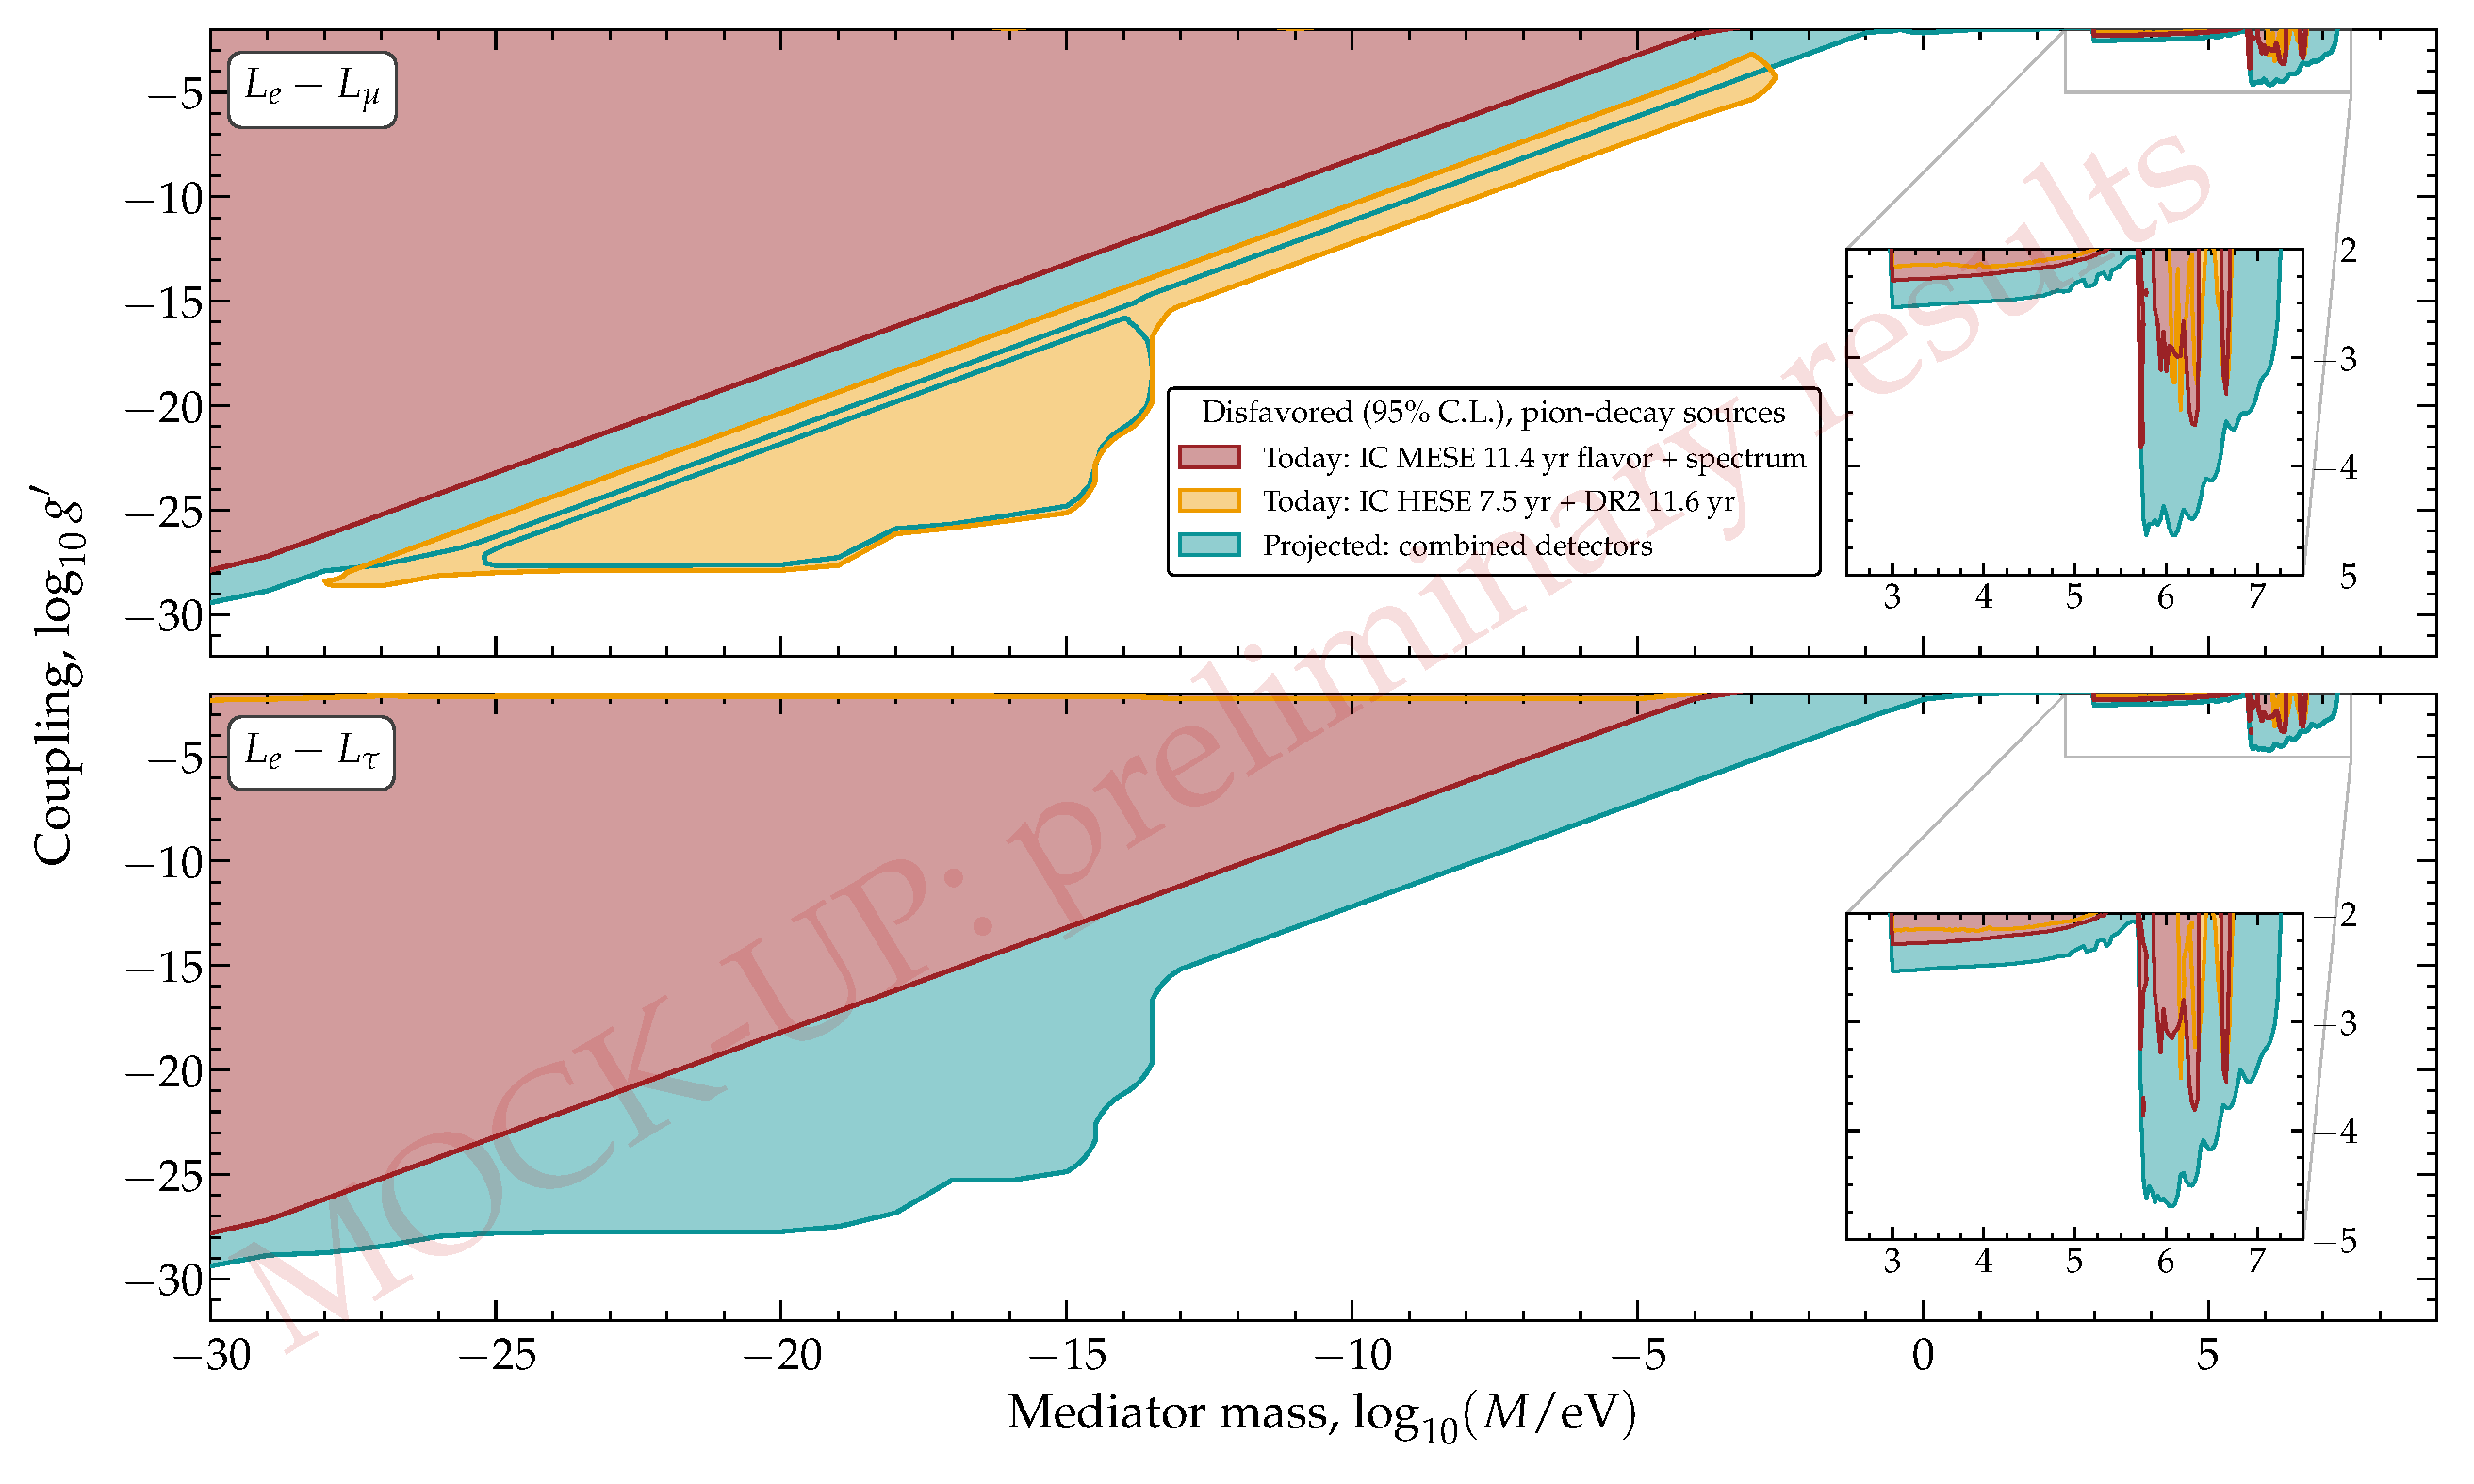
\includegraphics[width=\textwidth]{figures/mockup_fig4.pdf}
 % mock-up (watermarked, preliminary results; analysis/mockups.py), was: \placeholder{Fig.~4: $L_e - L_\mu$ and $L_e - L_\tau$, $10^{-30}$ to $10^9$~eV (after the final run).}
 \caption{\textbf{\textit{Limits on the coupling of the $L_e - L_\mu$ and $L_e - L_\tau$ gauge bosons, versus their mass.}} \textit{Top:} $L_e - L_\mu$. \textit{Bottom:} $L_e - L_\tau$. Each shaded region is disfavored at 95\%~C.L.\ by one data set, with sources of pion-decay composition. The insets enlarge the MeV masses, where absorption on the relics shapes the limits. Existing bounds are in gray (Table~\ref{tab:bounds}), and the region beyond perturbative unitarity is marked (Sec.~\ref{sec:models}). See Sec.~\ref{sec:results} for details. \todo{Takeaway from the final results.}}
 \label{fig:lelalpha}
\end{figure*}
%%%%%%%%%%%%%%%%%%%%%%%%%%%%%%%%%%%%%%%%%%%%%%%%%%%%%%%%

%%%%%%%%%%%%%%%%%%%%%%%%%%%%%%%%%%%%%%%%%%%%%%%%%%%%%%%%
\begin{figure*}[t!]
 \centering
 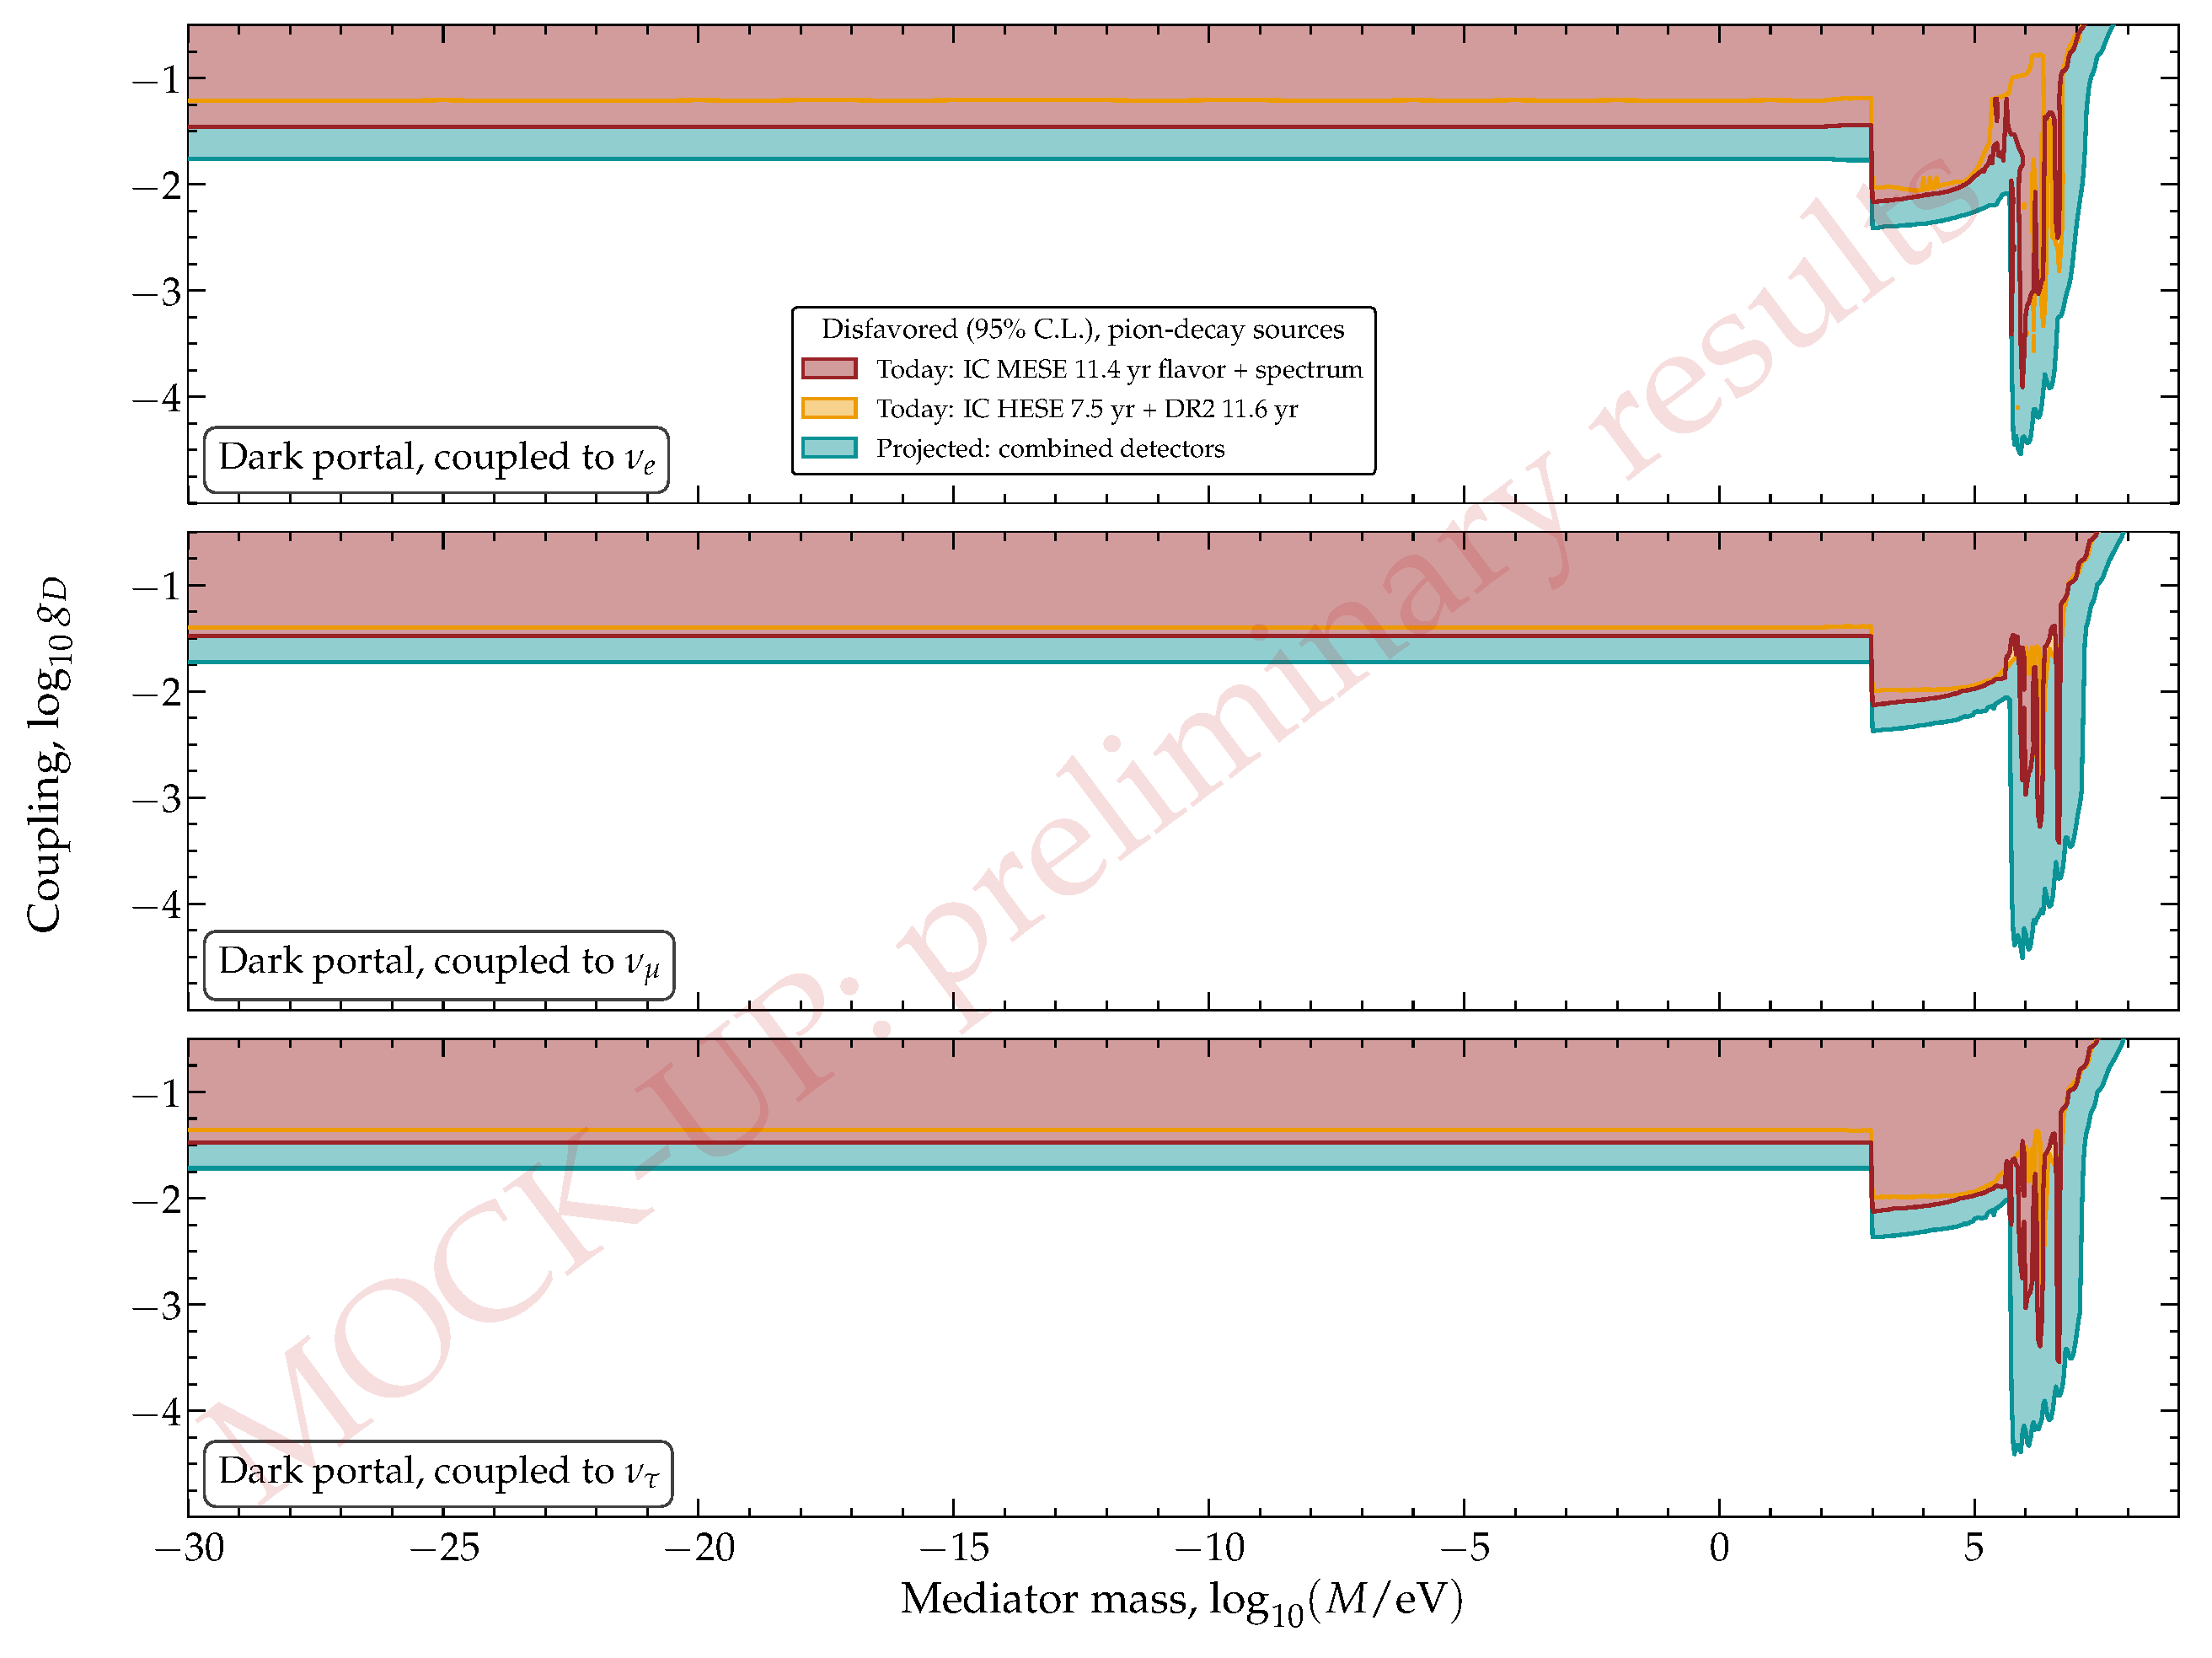
\includegraphics[width=\textwidth]{figures/mockup_fig5.pdf}
 % mock-up (watermarked, preliminary results; analysis/mockups.py), was: \placeholder{Fig.~5: the dark portal, textures $e$, $\mu$, $\tau$ (after the final run).}
 \caption{\textbf{\textit{Limits on the coupling of the dark-portal mediator, versus its mass, for each flavor it couples to.}} \textit{Top to bottom:} the mediator coupled to $\nu_e$, $\nu_\mu$, and $\nu_\tau$. Each shaded region is disfavored at 95\%~C.L.\ by one data set, with sources of pion-decay composition. See Sec.~\ref{sec:results} for details. \todo{Existing bounds (Table~\ref{tab:bounds}); takeaway from the final results.}}
 \label{fig:dp}
\end{figure*}
%%%%%%%%%%%%%%%%%%%%%%%%%%%%%%%%%%%%%%%%%%%%%%%%%%%%%%%%

%%%%%%%%%%%%%%%%%%%%%%%%%%%%%%%%%%%%%%%%%%%%%%%%%%%%%%%%
\begin{figure}[t!]
 \centering
 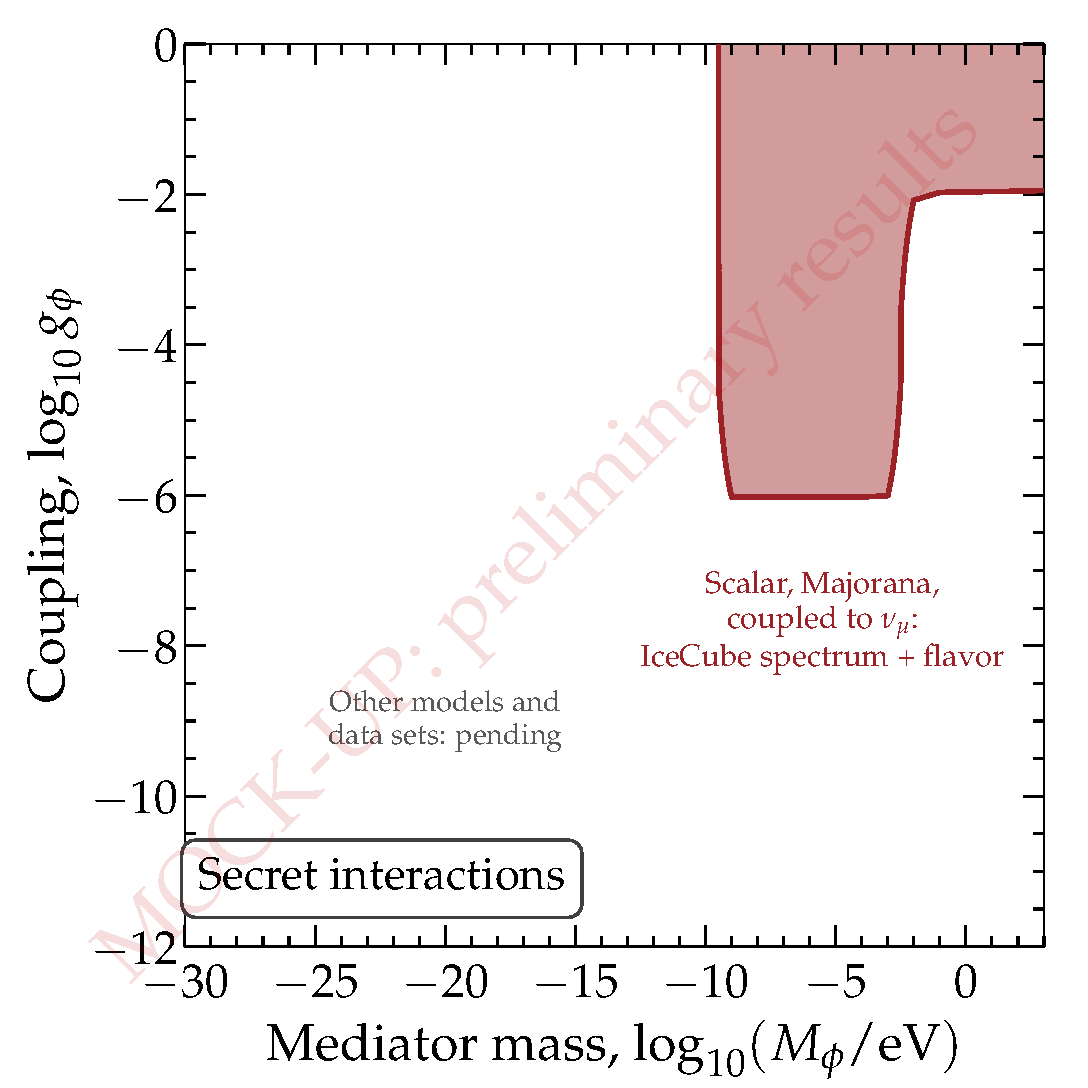
\includegraphics[width=\columnwidth]{figures/mockup_fig6.pdf}
 % mock-up (watermarked, preliminary results; analysis/mockups.py), was: \placeholder{Fig.~6: secret interactions (after the secret-interaction campaign).}
 \caption{\textbf{\textit{Limits on secret neutrino interactions, versus the mass of the mediator.}} \todo{Panels: scalar and vector, Majorana and Dirac, couplings to $\nu_e$, $\nu_\mu$, $\nu_\tau$, and to every flavor (after the secret-interaction run).} Each shaded region is disfavored at 95\%~C.L.\ by one data set. Existing bounds are in gray (Table~\ref{tab:bounds}). For the scalar, the region where the field that the relics source changes the neutrino masses, which we do not model, is marked (Sec.~\ref{sec:data}). See Sec.~\ref{sec:results} for details. \todo{Takeaway from the final results.}}
 \label{fig:si}
\end{figure}
%%%%%%%%%%%%%%%%%%%%%%%%%%%%%%%%%%%%%%%%%%%%%%%%%%%%%%%%

%%%%%%%%%%%%%%%%%%%%%%%%%%%%%%%%%%%%%%%%%%%%%%%%%%%%%%%%
\begin{figure}[t!]
 \centering
 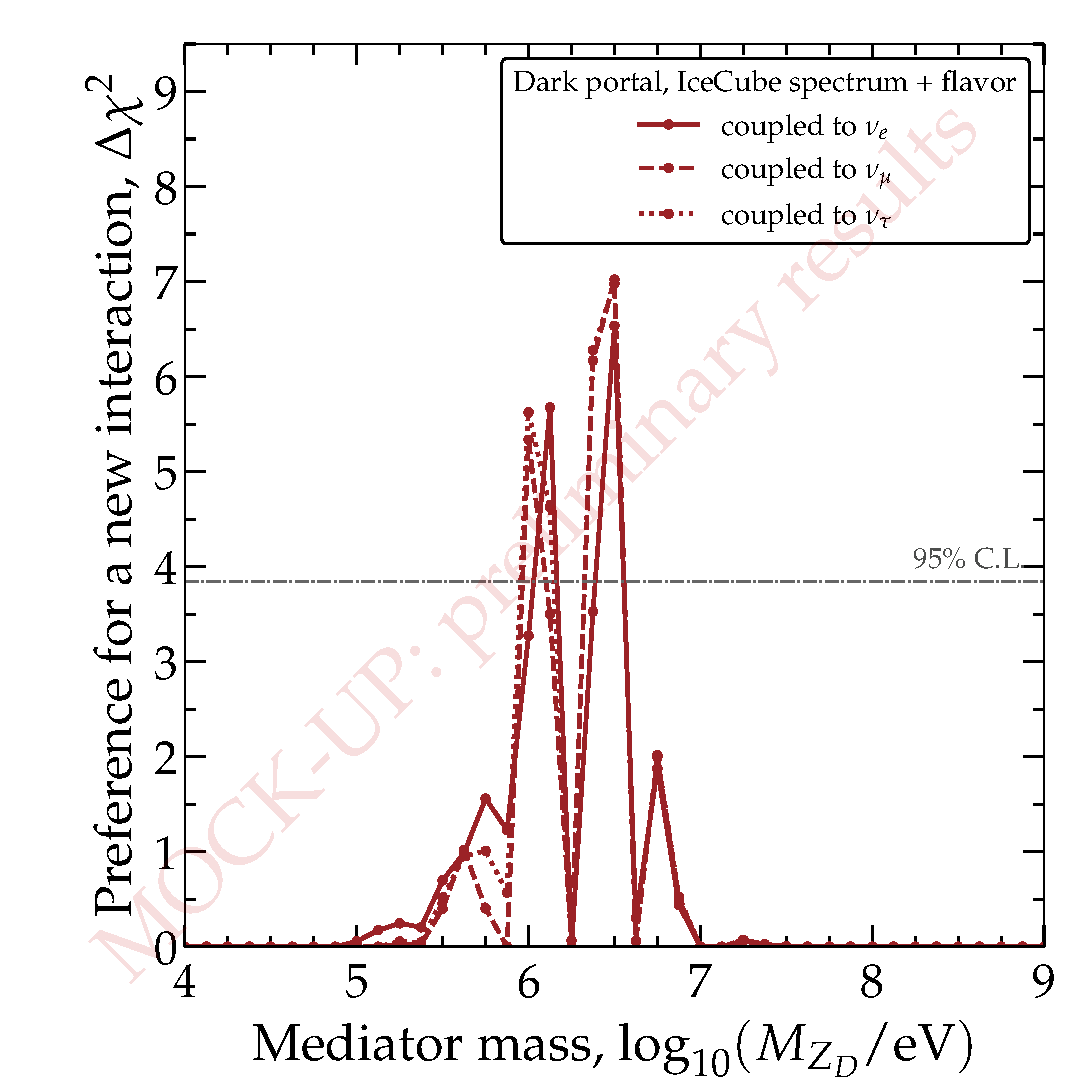
\includegraphics[width=\columnwidth]{figures/mockup_fig7.pdf}
 % mock-up (watermarked, preliminary results; analysis/mockups.py), was: \placeholder{Fig.~7: IceCube's MeV preference, or the discovery case.}
 \caption{\textbf{\textit{How much IceCube's spectrum and flavor composition prefer a dark-portal mediator to no new interaction, versus its mass.}} At each mass, the preference is the $\chi^2$ without a new interaction minus the lowest $\chi^2$ over the coupling. See Sec.~\ref{sec:results} for details. \todo{Final results: the masses and textures preferred, and the discovery case.}}
 \label{fig:discovery}
\end{figure}
%%%%%%%%%%%%%%%%%%%%%%%%%%%%%%%%%%%%%%%%%%%%%%%%%%%%%%%%

%%%%%%%%%%%%%%%%%%%%%%%%%%%%%%%%%%%%%%%%%%%%%%%%%%%%%%%%
%%%%%%%%%%%%%%%%%%%%%%%%%%%%%%%%%%%%%%%%%%%%%%%%%%%%%%%%
\section{Summary and outlook}
\label{sec:conclusions}

\todo{A recap for a fresh reader; main findings in bold; limitations; outlook; a closing statement that makes a new point.}

%%%%%%%%%%%%%%%%%%%%%%%%%%%%%%%%%%%%%%%%%%%%%%%%%%%%%%%%
%%%%%%%%%%%%%%%%%%%%%%%%%%%%%%%%%%%%%%%%%%%%%%%%%%%%%%%%
\appendix
% Figures and tables in the appendices numbered by appendix: Fig. A.1, Table B.1 (Mauricio, 2026-11-07)
\counterwithin{figure}{section}
\counterwithin{table}{section}
\renewcommand{\theHfigure}{\thesection.\arabic{figure}}
\renewcommand{\theHtable}{\thesection.\arabic{table}}

\section{The vertices of each model}
\label{app:vertices}
The transport works in the basis of neutrino mass states, $\nu_i$, related to the flavor states by $\nu_\alpha = \sum_i U_{\alpha i} \nu_i$.
For the vector mediators of Eqs.~(\ref{equ:lag_le}), (\ref{equ:lag_dp}), and (\ref{equ:lag_si}), the mass states couple through the Hermitian matrix $G' = U^\dagger G U$, with $G = g' \mathbf{S}_\alpha$ for $L_e - L_\alpha$.
For a scalar and Majorana neutrinos, they couple through the complex symmetric matrix $\lambda = U^T G U$.
This matrix is real only without CP violation.
For $\delta_{\rm CP} = 212^\circ$, even a flavor-universal coupling has off-diagonal entries of 1.1--13\% of $g$.
No rate depends on the Majorana phases.
When the scalar couples to a single flavor $\alpha$, so does $\delta_{\rm CP}$, since then $|\lambda_{ij}| = g\, |U_{\alpha i}| |U_{\alpha j}|$.
For a scalar and Dirac neutrinos, the coupling is $-\phi \sum_{ij} h_{ij}\, \bar\nu_i \nu_j$, with $h = U^\dagger G U$.
Since no observable fixes the mixing of the right-handed neutrinos, we give them that of the left-handed ones.

We evaluate the diagrams with Majorana neutrinos by the fermion-flow rules of Ref.~\cite{Denner:1992me}.
For Dirac neutrinos, the scalar changes chirality at each vertex, connecting a state that feels the weak interaction, $\nu_L$ or $\bar\nu_R$, with a sterile one, $\nu_R$ or $\bar\nu_L$.
A relic at rest presents both helicities to the high-energy neutrino.
Part of the secondaries of each collision are then sterile; the transport tracks them separately, per mass state and energy.

In the scalar's processes of Fig.~\ref{fig:processes}, each vertex joins two Majorana neutrinos, so a high-energy neutrino is absorbed on a relic neutrino, not on a relic antineutrino.

The longitudinal mode of a vector mediator couples through the divergence of its current.
For Majorana neutrinos, written as left-handed Weyl fields $\chi_i$, the current $\sum_{ij} G'_{ij}\, \chi_i^\dagger \bar\sigma^\mu \chi_j$ has divergence $i \sum_{ij} G'_{ij} (m_i \chi_i \chi_j - m_j \chi_i^\dagger \chi_j^\dagger)$.
At energies far above $M$, the longitudinal mode then acts as a scalar with the couplings $Y_{ij}$ of Eq.~(\ref{equ:goldstone}), through the term $-\frac{1}{2} \sum_{ij} Y_{ij}\, \phi\, \chi_i \chi_j + {\rm h.c.}$ in the Lagrangian~\cite{Allwicher:2021rtd}.
We require the largest eigenvalue of the tree-level partial-wave matrices of these couplings, for two-fermion states with total angular momentum $J = 0$ and for fermion-scalar states with $J = 1/2$, to stay below $1/2$ in magnitude~\cite{Allwicher:2021rtd}.


\section{The transport equation in full}
\label{app:transport}
This appendix gives every term of Eq.~(\ref{equ:transport}) after the sources, Eq.~(\ref{equ:source}), and the transport inside the Milky Way.
We write the terms for neutrinos; those for antineutrinos follow with each quantity replaced by its counterpart.

\subsubsection{Absorption and its secondaries}
The rate of absorption is that of Eq.~(\ref{equ:absorption}).
An absorption gives back one neutrino and one antineutrino.
The neutrinos returned into state $a$ at energy $E$ are
\begin{equation}
 \label{equ:secondaries}
 \begin{split}
 \mathcal{R}_a = \beta_a \int_E^\infty dE' \bigg[ & \frac{3E^2}{E'^3} \sum_c \Gamma^{\rm abs}_c F_c \\
 & + \frac{3(E'-E)^2}{E'^3} \sum_c \bar\Gamma^{\rm abs}_c \bar F_c \bigg]_{E'} \;,
 \end{split}
\end{equation}
where the first term comes from absorbed neutrinos and the second from absorbed antineutrinos.
The share of the secondaries that enter state $a$, $\beta_a = {\rm Re}(W^\dagger G G^\dagger W)_{aa} / [{\rm Tr}(G G^\dagger) + 24\pi\Gamma_{\rm vis}/M]$, follows from the coupling of the mediator to that state, with $\Gamma_{\rm vis}$ its width into charged leptons.
Summed over states, it is the branching ratio of the mediator into neutrinos.

\subsubsection{Scatterings on the relics}
They move neutrinos from state $a$ to state $b$ at the rate
\begin{equation}
 \label{equ:soft}
 R_{ba} = \Gamma_{\rm u}(z)\, |G_{ba}|^2\, \frac{\omega_{ab}^2}{\omega_{ab}^2 + D_{ab}^2} \;,
\end{equation}
where $G_{ba} = \langle b|G|a\rangle$, and $\omega_{ab}$ is the difference between the energies of the two states.
The damping $D_{ab}$ combines the rates at which scatterings and decays remove neutrinos from the two states.
When it exceeds the splitting $\omega_{ab}$, the conversions are suppressed.
The rate per unit coupling squared, $\Gamma_{\rm u}(z) \propto n_{\rm hel} (1+z)^3 / [M^2 + m_D^2(z)]$, grows with today's number density of relics in each mass state and helicity, $n_{\rm hel} = 3\zeta(3) T_{\nu,0}^3 / (4\pi^2)$, and falls with the mass of the mediator, increased by its screening mass $m_D$ in the gas of relics.

\subsubsection{Energy loss to relics that change mass}
A soft scattering $\nu_a \nu_r \to \nu_c \nu_s$ that leaves the relic in another mass state, $s \neq r$, has the same forward peak as the elastic one, since the relic keeps its light-cone momentum $p_r^- = E_r - p_{r\parallel}$, where $E_r$ is its energy and $p_{r\parallel}$ its momentum along the beam.
The beam neutrino pays for the change of mass, $\omega_{rs} = (m_s^2 - m_r^2)/(2 p_r^-)$ per scattering: it loses energy when the relic moves to a heavier state and gains it when the relic moves to a lighter one.
Once weighted with the flux factor $p_r^-/E_r$, this cost per unit time depends neither on the direction of the relic nor on the energy of the beam neutrino.
A neutrino in state $a$ thus loses observed energy at the rate
\begin{equation}
 \label{equ:loss}
 b_a(E, z) = \frac{C(z)\, (G G^\dagger)_{aa}}{1+z} \;,
\end{equation}
with
\begin{equation}
 \label{equ:loss_coeff}
 \begin{split}
 C(z) = \; & \frac{n_{\rm hel} (1+z)^3}{4\pi\, [M^2 + m_D^2(z)]} \\
 & \times \sum_{r \neq s} \eta_r\, |G'_{sr}|^2 \left( m_s^2 - m_r^2 \right) \left\langle \frac{1}{E_r} \right\rangle \;,
 \end{split}
\end{equation}
where $\eta_r$ is the occupation of relic state $r$ relative to that at production, which also sets its temperature, $T_{\nu,0} (1+z)\, \eta_r^{1/3}$, and the brackets average over its thermal energies.
Dirac relics couple to the vector only through their left-chiral share, so $\langle 1/E_r \rangle$ becomes $\langle (1+v_r)/(2E_r) \rangle$, with $v_r$ the speed of the relic.
The loss applies to the vector mediators below 1~keV: those of $L_e - L_\alpha$, the dark portal, and secret interactions.

Where the relics have decayed into $\nu_1$, we take them as $\nu_1$ alone, three times as many as in one state, in a hotter Fermi-Dirac gas that stands for the products of the decays.
Varying their number between one and three times that of one state, and $\langle 1/E_r \rangle$ by a factor of two either way, changes our limits only at $M = 10^{-2}$~eV, for the IceCube spectrum, where our choice gives the weaker limit.
In each step of the solution, the content of each energy bin moves down by its loss over the step and is spread over the bins that it then overlaps, which keeps the number of neutrinos exact except for those that cross the lowest energy of the grid.

\subsubsection{Decays}
State $a$ decays at the total rate
\begin{equation}
 \label{equ:decay_loss}
 \Gamma^{\rm dec}_a(E, z) = \sum_b \int_{x_-}^{x_+} dx\, \frac{d\Gamma_{a \to b}}{dx} \;,
\end{equation}
where $b$ runs over the open daughter states of neutrinos and antineutrinos alike, and the rates and kinematic limits are those of Appendix~\ref{app:decay}.
In vacuum, it is the sum of the rates $\Gamma_{i \to j}$ of the mass state, which fall as $m_i / [E(1+z)]$.
The daughters return to the flux as
\begin{equation}
 \label{equ:decay_gain}
 \mathcal{D}_a(E, z) = \sum_b \int_E^\infty \frac{dE'}{E'} \left. \frac{d\Gamma_{b \to a}}{dx} \right|_{x = E/E'} F_b(E') \;,
\end{equation}
where the rates vanish outside each window $x_- \leq x \leq x_+$, and the daughters that flip their helicity, for Majorana neutrinos, come from parents of the other kind.
The mediators that these decays emit enter Eq.~(\ref{equ:mediators}) through $\mathcal{P}_h$, the rate of decays that emit a mediator of helicity $h$ with the energy $(1 - x) E'$ of the parent that the daughter does not take.
Each mediator that decays adds its two daughters, with the energies of Appendix~\ref{app:decay}, to $\mathcal{M}_a$ and to its counterpart for antineutrinos.
Each decay of a neutrino keeps one neutrino, and each decay of a mediator adds two, so only the mediators change the number of neutrinos and antineutrinos.

In each step of the solution, we sweep down from the highest energy bin: the daughters of the bins above arrive first, then the populations of the bin decay, heaviest first, so that a chain such as $\nu_3 \to \nu_2 \to \nu_1$ completes within one step, exactly for any product of rate and step.
The daughters of a parent land on the bins that its window covers, through the exact integrals of their spectrum over each bin, which keeps the number of neutrinos exact except for those that fall below the lowest energy of the grid.
The relics decay as well; we describe their population after the decays with the energy loss, above.

\subsubsection{The Milky Way}
Inside the Galaxy, the number $G_a(E, \ell, \hat n)$ of neutrinos that travel toward the Sun along direction $\hat n$, at distance $\ell$ from it, evolves as
\begin{equation}
 \label{equ:galactic}
 \begin{split}
 -\frac{\partial G_a}{\partial \ell} = \; & j_a + \sum_{b \neq a} \left( R_{ab} G_b - R_{ba} G_a \right) \\
 & + \frac{\partial}{\partial E} \left( b_a G_a \right) - \Gamma^{\rm dec}_a G_a + \mathcal{D}_a \;,
 \end{split}
\end{equation}
with every rate evaluated today, in the eigenstates of the local potential.
Absorption is left out: the Galaxy holds a column of relics about $10^{-5}$ times that of the Universe.
The Galaxy emits, per unit length,
\begin{equation}
 \label{equ:emission}
 \begin{split}
 j_a = \; & \tfrac{3}{2}\, N_{\rm G}\, I(E, \hat n) \left[ w_{\rm gas}\, q_{\rm gas}(\ell, \hat n) + (1 - w_{\rm gas})\, q_{\rm src}(\ell, \hat n) \right] \\
 & \times \sum_\alpha f_\alpha\, |\langle\nu_\alpha|a\rangle|^2 \;,
 \end{split}
\end{equation}
where $I$ is the intensity per flavor, neutrinos plus antineutrinos, of the template of Ref.~\cite{Schwefer:2022zly}, so that the factor $3/2$ gives all three flavors of one kind.
The normalization $N_{\rm G}$ is free in the fits; $w_{\rm gas}$ is the share of the emission from the gas.
The distributions $q_{\rm gas}$ and $q_{\rm src}$ of the emission from the gas and from unresolved sources along the line of sight are normalized to one; $(f_e, f_\mu, f_\tau) = (x, 1-x, 0)$ is the flavor composition at emission.
Where the Galactic potential allows decays that the cosmological potential forbids, the extragalactic flux crosses the Galaxy by the same equation without emission, along every line of sight, and is then averaged within each band of declination.

\subsubsection{Numerical solution}
We solve Eq.~(\ref{equ:transport}) on energies spaced uniformly in $\ln E$, 0.02 apart, up to 30~PeV.
The grid starts at 4.6~TeV for the measurements of the spectrum and the flavor composition, at 1.0~TeV for the event samples, and at 99~GeV for the future telescopes.
In every transport, the grid extends to ten times 30~PeV, so that the neutrinos injected above 30~PeV, and the daughters and secondaries that fall from there, enter it.
The cosmological transport takes 200 steps in redshift, from $z = 4$ to today, and 400 where neutrinos decay: where decays and scatterings act together, 200 steps leave up to $6 \times 10^{-3}$ in the shape of the spectrum, and 400 at most $1.7 \times 10^{-3}$.
The collision transport takes steps uniform in $\ln(1+z)$, one per energy bin above 1~keV and two below.
Against 800 steps, without decays, the two transports give 0.5\% more and 0.17\% less flux, respectively, at every energy alike, which the free normalization of the flux absorbs.

The eigenstates depend on energy and redshift only through $\sigma$, so we tabulate them on a grid in $\sigma$; for the cosmological transport, about 4000 nodes reproduce the eigenvectors computed directly to $2.7 \times 10^{-14}$.
We interpolate between solutions at three values of each spectral index (seven for the upper index in the planes of MeV mediators), which is accurate to 0.35\% in the flux and to $9 \times 10^{-4}$ in the flavor fractions.
We compute the flux in 768 directions, the pixels of HEALPix with $N_{\rm side} = 8$~\cite{Gorski:2004by}.
Past the Sun, we follow 8 paths, at the Gauss-Legendre nodes in the cosine of the angle to the Sun, with nodes close enough that the eigenbasis turns by at most 0.002 between them.
Through the Earth, we follow 12 chords in each band of declination (Appendix~\ref{app:earth}).

\section{The flux at each stage of propagation}
\label{app:stops}

Figure~\ref{fig:trip} shows the flux and its flavor composition at four stops of the trip, from 10~TeV to 30~PeV: as it reaches the Milky Way, after crossing it, near the Earth, and at the detector.
Its top row shows the flux of all flavors relative to that on arrival at the Milky Way; the rows below show the fraction of each flavor.
Its two columns are the masses of $L_e - L_\mu$ in Fig.~\ref{fig:species}, with the same couplings.
It complements Fig.~\ref{fig:species}, which follows one energy along the trip: at $10^{-20}$~eV, the flavor composition changes at the stop near the Earth; at $10^{-26}$~eV, at the stop after the Milky Way, where the flux also drops.

%%%%%%%%%%%%%%%%%%%%%%%%%%%%%%%%%%%%%%%%%%%%%%%%%%%%%%%%
\begin{figure*}[t!]
 \centering
 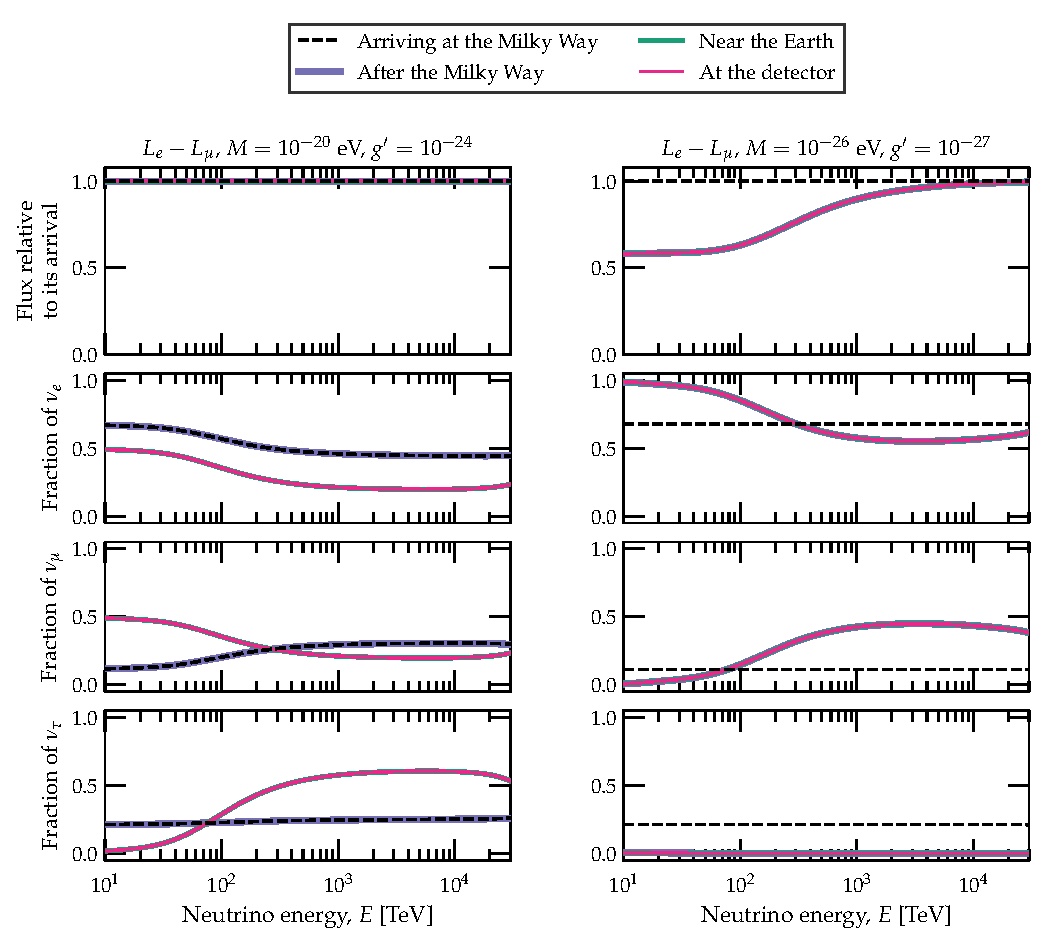
\includegraphics[width=\textwidth]{figures/flux_stops.pdf}
 \caption{\textbf{\textit{Flux and flavor composition of high-energy neutrinos at the stops of their trip.}} \textit{Top:} the flux of all flavors, neutrinos plus antineutrinos, relative to its value on arrival at the Milky Way. \textit{Below:} the fraction of each flavor. The sources emit $\nu_e : \nu_\mu : \nu_\tau = 1 : 2 : 0$ with a spectrum $E^{-2.5}$; the neutrino masses follow the normal ordering, with a lightest mass of $10^{-6}$~eV. See Sec.~\ref{sec:trip} and Appendix~\ref{app:stops} for details. Which stop shapes the flux depends on the range of the mediator: the Sun, for $M = 10^{-20}$~eV, and the Milky Way, for $M = 10^{-26}$~eV.}
 \label{fig:trip}
\end{figure*}

%%%%%%%%%%%%%%%%%%%%%%%%%%%%%%%%%%%%%%%%%%%%%%%%%%%%%%%%
\section{Thermal absorption rates and the relics' helicity}
\label{app:thermal}
Absorption on a relic of mass $m_r$ is a resonance at $s = M^2$, where $s$ is the square of the energy of the collision in its center-of-momentum frame.
For a relic at rest, $s = 2E(1+z)\, m_r$.
The relics, however, move, with Fermi--Dirac momenta at the temperature $T_{\nu,0}(1+z)$.
A relic of energy $E_p$ and momentum $p$ that meets the high-energy neutrino at an angle $\theta$ gives $s = m_r^2 + 2E(1+z)\, \epsilon$, with $\epsilon = E_p - p\cos\theta$.
Thus, the motion of the relics spreads the resonance over a range of energies, most of all for a relativistic lightest relic~\cite{Wang:2025qap}.
The resonance is far narrower than any grid in energy, so we integrate the Breit--Wigner rate over the momenta of the relics semi-analytically, treating the narrow zone around the resonance with exact antiderivatives.
For a vector coupled to left-handed neutrinos, the width of the mediator is $\Gamma = M\, {\rm Tr}(G G^\dagger) / (24\pi)$, plus its width into charged leptons where those decays are open.

At MeV masses, we average every term of the collision over the momenta of the relics, not only the resonance.
Each product of a collision is boosted along the incoming neutrino by a Lorentz factor of about $E/\sqrt{s} \sim 10^8$.
Its share of the energy is the same in the frame of the relic as in the cosmological frame, so the energy spectra of the products depend on $s$ alone.
Averaging over the momenta of the relics then reduces to averaging over $s$.

A Dirac relic retains its helicity from the time of decoupling: $-1/2$ for a neutrino and $+1/2$ for an antineutrino.
At rest and averaged over directions, it is unpolarized; in motion, its spin follows its momentum.
The spin of a relic neutrino along the direction of the incoming neutrino is
\begin{equation}
 \label{equ:polarization}
 \pi = \frac{E_p\, \epsilon - m_r^2}{p\, \epsilon} \;,
\end{equation}
from $-1$ for a relic that moves along with the incoming neutrino to $+1$ for one that moves against it.
After averaging over the azimuth of the final state, the squared amplitude of a collision is
\begin{equation}
 \label{equ:helicity_mix}
 |\mathcal{M}|^2 = \frac{1 + \pi}{2}\, |\mathcal{M}_L|^2 + \frac{1 - \pi}{2}\, |\mathcal{M}_R|^2 \;,
\end{equation}
up to terms of order $m_r^2/s$, where $\mathcal{M}_L$ and $\mathcal{M}_R$ are the amplitudes for a massless relic of left- or right-handed chirality at the same $s$.
A vector couples only to the left-handed part; a scalar couples to both, with the visible and sterile secondaries of Appendix~\ref{app:vertices}.
We take the density of relics everywhere as the cosmological mean, neglecting their clustering in the Milky Way~\cite{Ringwald:2004np, deSalas:2017wtt, Mertsch:2019qjv}.

Figure~\ref{fig:helicity} shows the consequences for a $\nu_e$-coupled mediator, with Dirac neutrinos: the flux over that with no new interaction, versus energy, for a scalar (top) and a vector (bottom), at $M = 31.6$~keV with $g = 2 \times 10^{-3}$ and $M = 4.22$~MeV with $g = 1.35 \times 10^{-3}$ (left and right), for lightest neutrino masses of $10^{-6}$~eV (thick lines) and 0.03~eV (thin lines).
Its lines compare relics at rest, relics in motion without their helicity, and relics in motion with it.
With a relativistic lightest relic, the helicity matters most: the scalar's resonance on it nearly disappears, while the vector's deepens.

%%%%%%%%%%%%%%%%%%%%%%%%%%%%%%%%%%%%%%%%%%%%%%%%%%%%%%%%
\begin{figure*}[t!]
 \centering
 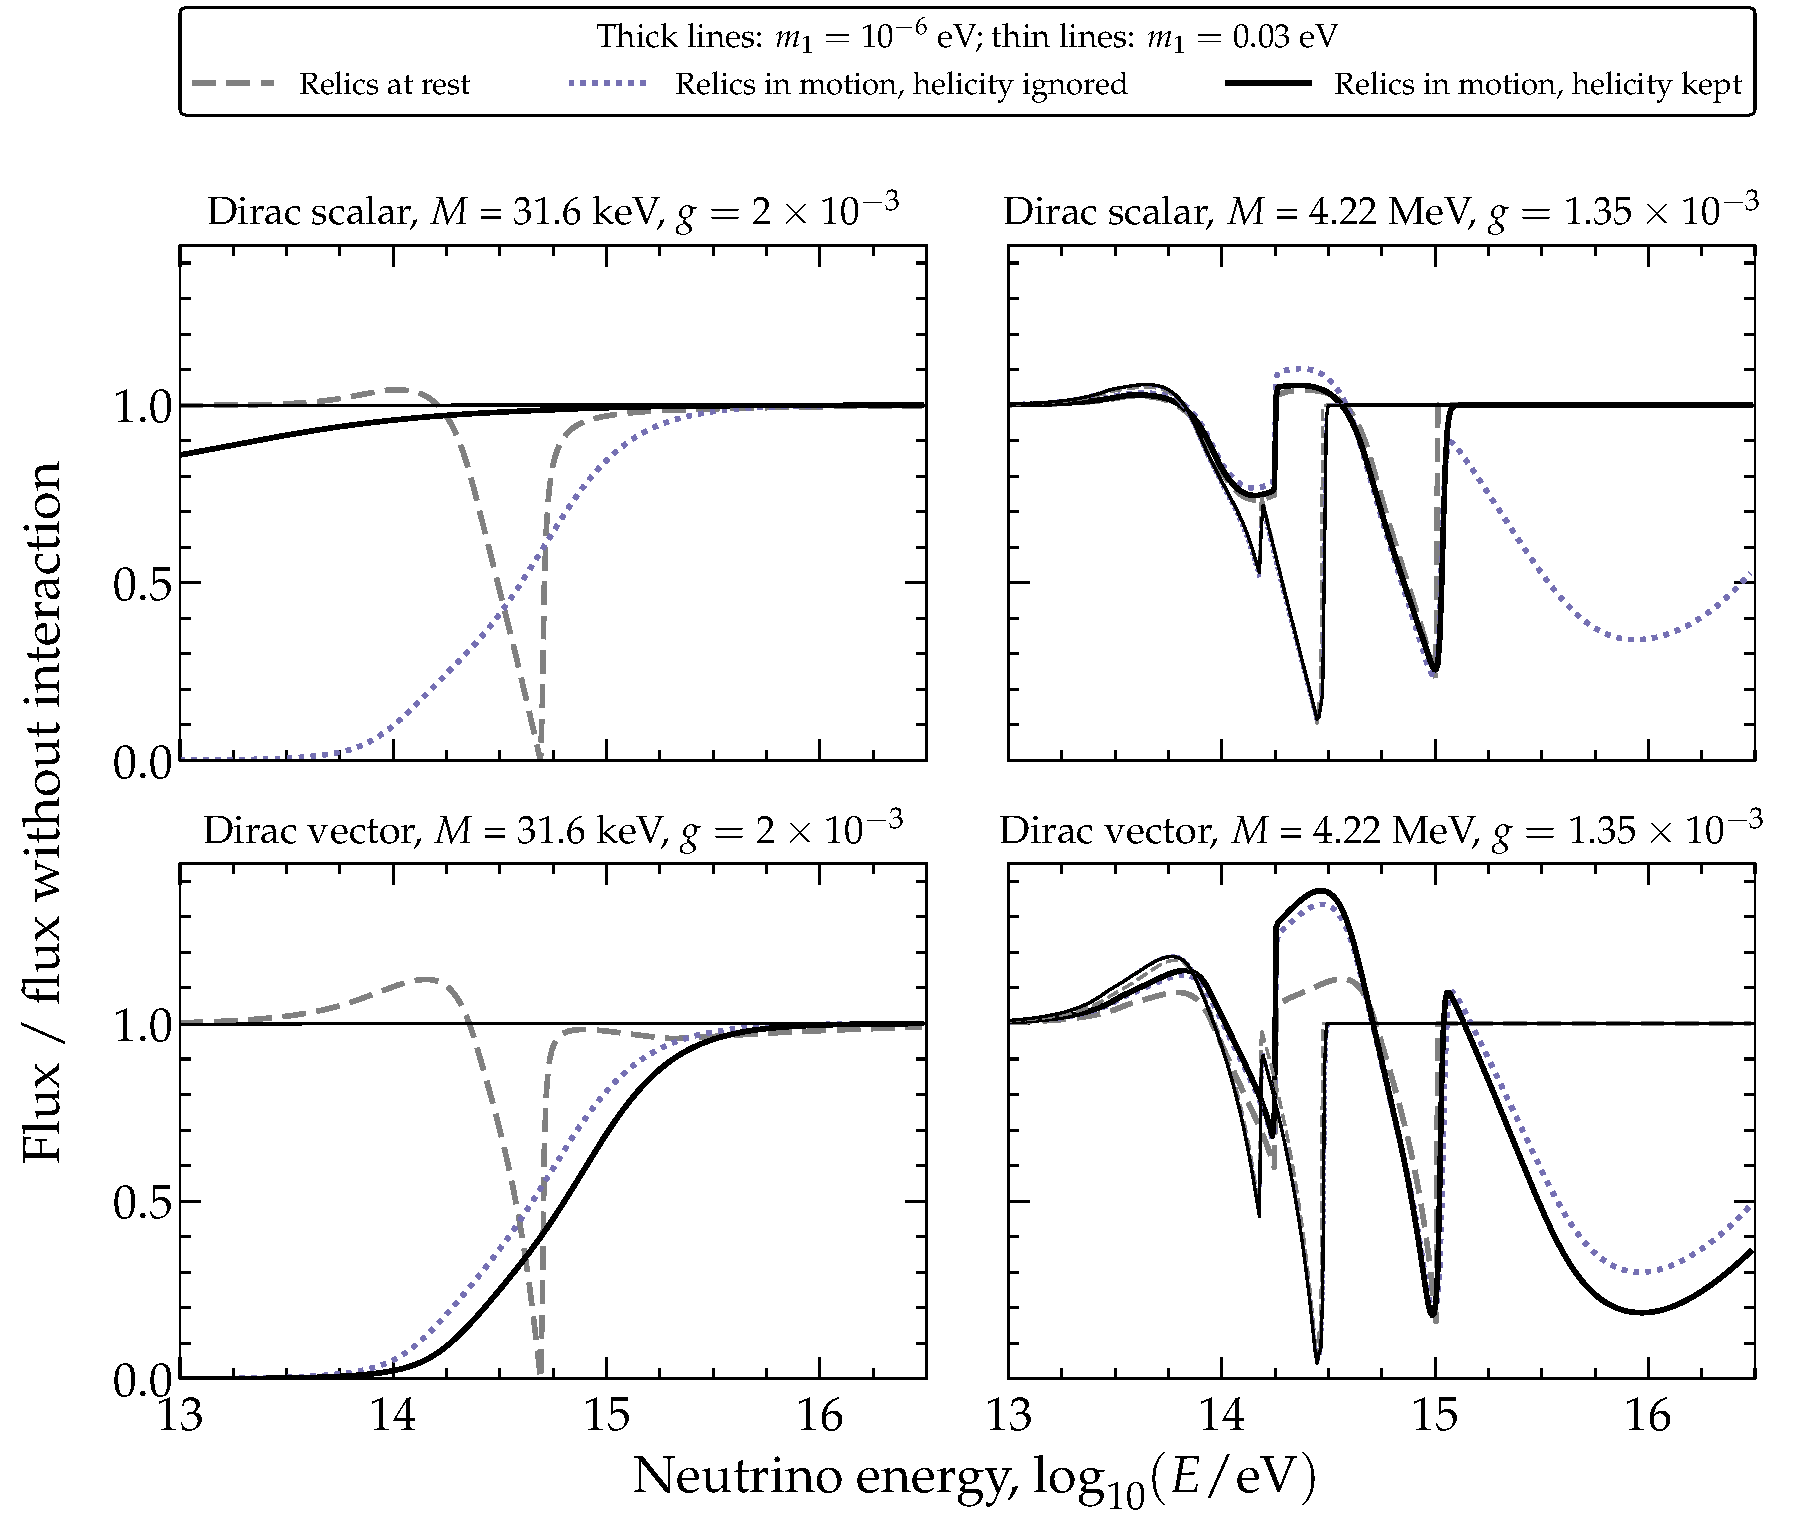
\includegraphics[width=0.9\textwidth]{figures/dirac_relic_helicity.pdf}
 \caption{\textbf{\textit{Flux of high-energy neutrinos with secret interactions on Dirac relic neutrinos, with and without the helicity of the relics.}} The flux relative to that without a new interaction, for a mediator coupled to $\nu_e$. The helicity matters most for a relativistic lightest relic: for the scalar, the resonance on it nearly disappears; for the vector, it deepens. See Appendix~\ref{app:thermal} for details.}
 \label{fig:helicity}
\end{figure*}
%%%%%%%%%%%%%%%%%%%%%%%%%%%%%%%%%%%%%%%%%%%%%%%%%%%%%%%%

\section{Decays in a medium}
\label{app:decay}
A neutrino $\nu_i$ decays into a lighter $\nu_j$ and the mediator when $m_i > m_j + M$ [Fig.~\ref{fig:processes}(g)].
In vacuum, a neutrino of observed energy $E'$ at redshift $z$ decays at the rate $\Gamma_{i \to j} = \Gamma^{\rm rest}_{ij}\, m_i / [E'(1+z)]$, with $\Gamma^{\rm rest}_{ij}$ the rate at rest.
The daughter takes a fraction $x = E/E'$ of its parent's energy, distributed as
\begin{equation}
 \label{equ:daughters}
 \frac{d\Gamma^{\rm keep,\,flip}_{i \to j}}{dE} = \frac{\Gamma_{i \to j}}{E'} \left[ a + b\, x + \frac{c}{x} \right]^{\rm keep,\,flip}_{ij}
\end{equation}
between the kinematic limits $x_-$ and $x_+$, with coefficients $a$, $b$, $c$ that follow from the helicity amplitudes of the decay.
The daughter keeps the helicity of its parent (``keep'') or, for Majorana neutrinos, flips it and emerges as an antineutrino (``flip'').
Every decay keeps one neutrino, so decays conserve the number of neutrinos while they lower their energy.

Inside a potential, decays connect the eigenstates of Eq.~(\ref{equ:hamiltonian}), since those are the states in which the neutrinos propagate.
Writing the potential as $\mathbf{V} = A\, \mathbf{S}$, the eigenvalues of ${\rm diag}(m_i^2) + \sigma\, U^\dagger \mathbf{S} U$, with $\sigma = 2E(1+z) A$, are the effective squared masses $\mu_a(\sigma)$.
A parent in state $a$ with energy $E'$ yields a daughter in state $b$ with energy $xE'$; parent and daughter are projected on their own eigenvectors, evaluated at $\sigma$ and $x\sigma$, respectively.
Energy conservation fixes the transverse momentum of the daughter,
\begin{equation}
 \label{equ:window}
 k_T^2 = (1 - x) \left[ x\, \mu_a(\sigma) - \mu_b(x\sigma) \right] - x M^2 \geq 0 \;,
\end{equation}
and the rate is $d\Gamma_{a \to b}/dx = |\mathcal{A}_{a \to b}|^2 / [16\pi E'(1+z)]$, with the amplitude
\begin{equation}
 \label{equ:medium_amp}
 \mathcal{A}_{a \to b} = \sum_{ij} c^*_{jb}(x\sigma)\, c_{ia}(\sigma)\, \mathcal{V}_{ji} \;.
\end{equation}
Here, $c_{ia} = \langle\nu_i|a\rangle$ and $\mathcal{V}_{ji}$ is the vacuum amplitude for $\nu_i$ to decay into $\nu_j$ and the mediator.
The potential does not act as a mass in the amplitude; it enters only through the eigenvectors and the kinematic window.
A state cannot decay into itself or into a state of the same kind that lies above it, so the lowest state of each kind decays only by flipping its helicity.
A potential also opens the decay of a neutrino state into the antineutrino state with the same label, which is closed in vacuum.
Without a potential, these rates reduce to those of Eq.~(\ref{equ:daughters}).

This treatment is valid as long as the width of every state stays well below its separation from the other states in effective mass squared, \ie, as long as $\zeta_a = 2E'(1+z)\, \Gamma_a / \min_b |\mu_a - \mu_b| \ll 1$; the corrections are of order $\zeta_a$.
Near the line of perturbative unitarity, at $g/M$ of 10 to 100~eV$^{-1}$, $\zeta_a$ reaches 0.1--0.5, so the decay rates there are uncertain by that fraction.
\todo{The outcome of the mapping of $\zeta_a$ in the final run.}

The mediators that these decays emit can decay in turn.
When the mediator is heavier than two neutrinos, $M > m_k + m_l$, it decays in flight into the pair $\nu_k \nu_l$ [Fig.~\ref{fig:processes}(f)].
The decay returns the mediator's energy to the flux, as neutrinos and antineutrinos with less energy than the neutrino that emitted it.
We follow these mediators by helicity, which sets how the energy divides between the two daughters: three populations for a vector mediator and one for a scalar, which decays isotropically.
A mediator of observed energy $E'$ decays at the rate $\Gamma_{\rm med}\, M / [E'(1+z)]$ whatever its helicity, where $\Gamma_{\rm med}$ is its width at rest into neutrino pairs.
Its helicity at emission and the energies of its daughters follow from the helicity amplitudes of the two decays.
We take the mediators still alive today as invisible; across the Milky Way, they would decay about $10^{-5}$ times as much as over their cosmological trip.
For Dirac neutrinos, a scalar decays into one active and one sterile neutrino; a vector decays into two active ones.

Emission and decay in flight occur together, at couplings near our limits, only for $M$ between about $9 \times 10^{-3}$ and $5 \times 10^{-2}$~eV, where only $\nu_3$ can emit the mediator.
At smaller masses, they occur only at couplings two to four orders of magnitude above our limits.
At $M = 10^{-2}$~eV and a coupling of $10^{-5}$, the decay back nearly doubles the flux at Earth.
\todo{Where it moves the limits: the outcome of the check.}

We neglect decays from the Sun on.
There, they change a state by more than $10^{-3}$ only where the flavor already follows the potential, at $\sigma / \Delta m^2_{21} \geq 840$ in the Sun and $\geq 3.4 \times 10^5$ in the Earth; the lowest states, as which the flux arrives, never decay there.

\section{The collision terms in full}
\label{app:si}
Where the potential is negligible, as for mediators above 1~keV and for secret interactions at every mass, the eigenstates of Eq.~(\ref{equ:hamiltonian}) are the mass states, and $F_i(E, z)$ counts the neutrinos per unit energy in $\nu_i$.
There we write the collision terms of Eq.~(\ref{equ:transport}), $-\Gamma^{\rm abs}_i F_i + \mathcal{R}_i + \sum_{j \neq i} (R_{ij} F_j - R_{ji} F_i)$, together, as
\begin{equation}
 \label{equ:collisions}
 \begin{split}
 \mathcal{C}_i(E, z) = \; & -\Gamma_i F_i \\
 & + \sum_j \int_E^\infty dE'\, K_{ij}(E, E')\, \Gamma_j(E')\, F_j(E') \;,
 \end{split}
\end{equation}
where $\Gamma_i$ is the total rate of collisions on the relics, and $K_{ij}(E, E')$ is the energy spectrum of the neutrinos in state $i$ that a collision of $\nu_j$ with energy $E'$ produces.
The energy loss, the decays, and the mediators that the decays emit keep their terms in Eq.~(\ref{equ:transport}).
For Majorana neutrinos, one population holds both helicities of each mass state, since the interaction treats them alike; we split it between neutrinos and antineutrinos in the proportions of the sources.
For Dirac neutrinos, we follow the visible and the sterile states of each mass state separately, six populations in all.
The rate $\Gamma_i$ sums the $s$, $t$, and $u$ channels, their interferences, and pair production [Fig.~\ref{fig:processes}(b)--(e)], each averaged over the momenta of the relics (Appendix~\ref{app:thermal}).
Each collision between two neutrinos produces two neutrinos.
Each pair production produces four when the mediators decay into neutrinos, which they do at once.
The products of the $t$ and $u$ channels at small momentum transfer return close to the incident energy; we treat their return as a drift in energy rather than as a transfer between energy bins.

For the scalar, we take the cross sections of Ref.~\cite{Esteban:2021tub}, Appendix~A, with two corrections.
First, the Majorana mass states couple through the complex matrix $\lambda = U^T G U$ (Appendix~\ref{app:vertices}), which Ref.~\cite{Esteban:2021tub} takes as real; the two agree only without CP violation.
Second, pair production sums the exchanged mass states coherently, which changes its cross section by factors of 0.08 to 2 with respect to the printed form.
For the vector, we derive the cross sections from Eq.~(\ref{equ:lag_si}).
We checked every cross section against an explicit computation of the amplitudes with Dirac matrices and helicity spinors.

We use these collision terms for secret interactions at every mass, and for the dark portal and $L_e - L_\alpha$ at MeV masses, where their potential is negligible.
Below 1~keV, they also carry the dark portal's and $L_e - L_\alpha$'s scatterings with large momentum transfer, for couplings above $10^{-4}$.

\section{The Earth's chords}
\label{app:earth}
A neutrino that reaches the detector from zenith angle $\theta_z$ crosses a chord of the Earth or, from above, only the ice over the detector.
Along each chord, we evolve the density matrix by Eq.~(\ref{equ:coherent}) in steps.
Each step takes the exact mean density of the Preliminary Reference Earth Model~\cite{Dziewonski:1981xy} over its length, computed layer by layer.
When the range of the mediator approaches the thickness of a layer, we use instead the density smoothed by the Yukawa factor of Eq.~(\ref{equ:potential}), which relaxes across each boundary between layers over a length $1/M$.
The phase accumulated by the potential then equals its integral along the chord, whatever the number of steps; we use 25.
The same integral gives the Earth's potential at the detector and, where the range exceeds the radius of the Earth, outside it.

We average the chords over the sky with equal weight per $\cos\theta_z$, within each band of declination.
At MeV masses, the potential accumulates a phase of $10^5$ to $10^8$~rad across the Earth, so the off-diagonal blocks of the density matrix oscillate rapidly from chord to chord.
An equal-weight mean over a finite set of chords would keep these oscillations as noise.
Instead, we integrate each block against its phase over $\cos\theta_z$, which reproduces the exact average over the sky to $10^{-5}$.

\section{Existing bounds}
\label{app:bounds}
Table~\ref{tab:bounds} lists the bounds of other works that Figs.~\ref{fig:lelalpha}--\ref{fig:si} show in gray, with their sources and confidence levels.
We read most of them off the figures of their sources, from the curves stored in the PDF files of those papers, with the axes calibrated on the drawn tick marks.
Each bound keeps the confidence level of its source, which varies from one bound to the next and is not always stated.
For this reason, we show them for orientation only and do not combine them with our limits.

We express every bound in terms of our couplings.
For $L_e - L_\alpha$, the couplings of Refs.~\cite{Coloma:2020gfv, Dror:2020fbh, Bauer:2018onh} equal our $g'$.
For secret interactions, those of Refs.~\cite{Blinov:2019gcj, Brdar:2020nbj} equal our $G_{\alpha\beta}$.
The compilation of Ref.~\cite{Berryman:2022hds} does not state its normalization; its laboratory bounds on $G_{ee}$ and $G_{\mu\mu}$ coincide with those of Ref.~\cite{Blinov:2019gcj} to within 0.05 in $\log_{10} G_{\alpha\beta}$, so we take it to be the same.

We compute two bounds ourselves.
First, we obtain the laboratory bounds on $L_e - L_\alpha$ with DarkCast~\cite{Ilten:2018crw, Baruch:2022esd}, which recasts the limits of searches for dark photons, and of other laboratory measurements, into other models; its coupling equals our $g'$.
Second, we apply the CMB bound on the lifetime of a neutrino that decays into a lighter one and a massless scalar, $\tau_i > 1.3 \times 10^9~{\rm s}\, (m_i / 0.05~{\rm eV})^3$ at 95\%~C.L., from the Planck 2018 data~\cite{Escudero:2019gfk}.
We apply it to the vacuum decay rates of Appendix~\ref{app:decay} in the $L_e - L_\alpha$ and dark-portal models, for mediators of any spin and of any mass that the decay allows (our extrapolation).
At each mediator mass, we take the most constraining neutrino state and then the weakest bound over lightest neutrino masses between $10^{-6}$ and 0.1~eV.

%%%%%%%%%%%%%%%%%%%%%%%%%%%%%%%%%%%%%%%%%%%%%%%%%%%%%%%%
\begin{table*}[t]
 \caption{\textbf{\textit{Existing bounds shown in gray in Figs.~\ref{fig:lelalpha}--\ref{fig:si}.}} For secret interactions, the bounds are on a scalar mediator and Majorana neutrinos, on the coupling of each panel of Fig.~\ref{fig:si} unless the row names one. ``Not stated'' marks a confidence level that the source does not give. See Appendix~\ref{app:bounds} for how each bound was obtained.}
 \label{tab:bounds}
 \begin{ruledtabular}
 \begin{tabular}{>{\raggedright\arraybackslash}p{0.47\textwidth}>{\raggedright\arraybackslash}p{0.27\textwidth}>{\raggedright\arraybackslash}p{0.18\textwidth}}
 Bound & Source & Confidence level \\
 \hline
 \multicolumn{3}{l}{\textit{$L_e - L_\mu$ and $L_e - L_\tau$}} \\
 Oscillations, global fit & \cite{Coloma:2020gfv} & $2\sigma$ \\
 Fifth-force searches, equivalence-principle tests & Recast in Ref.~\cite{Coloma:2020gfv} & As in the recast searches \\
 Planetary precession & \cite{KumarPoddar:2020kdz} & \todo{check} \\
 Black-hole superradiance (mass ranges) & \cite{Baryakhtar:2017ngi} & --- \\
 Meson decays; $0\nu\beta\beta$ with emission of the mediator; BBN and supernovae; decay of solar neutrinos & \cite{Dror:2020fbh} & Not stated \\
 White-dwarf cooling; matter effects in Super-Kamiokande & \cite{Bauer:2018onh} & Not stated \\
 Laboratory searches & DarkCast~\cite{Ilten:2018crw, Baruch:2022esd} & As in each search \\
 CMB, neutrino lifetime & \cite{Escudero:2019gfk}, with our decay rates & 95\% \\
 High-energy flavor composition, earlier estimate & \cite{Agarwalla:2023sng} & 95\% \\
 \hline
 \multicolumn{3}{l}{\textit{Dark portal}} \\
 CMB, neutrino lifetime & \cite{Escudero:2019gfk}, with our decay rates & 95\% \\
 \hline
 \multicolumn{3}{l}{\textit{Secret interactions}} \\
 Laboratory & \cite{Blinov:2019gcj} & Not stated \\
 $Z$ invisible width; $\tau$ decays & \cite{Brdar:2020nbj} & $3\sigma$ \\
 BBN, excluding $M < 1.3$~MeV & \cite{Blinov:2019gcj} & 95\% \\
 $0\nu\beta\beta$ with emission of the mediator ($G_{ee}$) & \cite{Berryman:2022hds}, from Ref.~\cite{Brune:2018sab} & As in the source \\
 IceCube HESE, 7.5~yr ($G_{\tau\tau}$) & \cite{Esteban:2021tub} & As in the source \\
 SN 1987A, propagation and core (equal $G_{\alpha\alpha}$) & \cite{Shalgar:2019rqe, Kolb:1987qy} & As in the sources \\
 CMB; TXS 0506+056 (equal $G_{\alpha\alpha}$) & \cite{Archidiacono:2013dua, Kelly:2018tyg} & As in the sources \\
 IceCube HESE, 6~yr (equal $G_{\alpha\alpha}$) & \cite{Bustamante:2020mep} & As in the source \\
 \end{tabular}
 \end{ruledtabular}
\end{table*}
%%%%%%%%%%%%%%%%%%%%%%%%%%%%%%%%%%%%%%%%%%%%%%%%%%%%%%%%

\bibliography{references}

\end{document}
